\documentclass[12pt,a4paper]{article}
 
\usepackage{float}
%für feststellen der figures und tables [H] dranschreiben
\usepackage{units}
%wird so benutzt: 
%\unit[value/Zahl]{dimension/Einheit} oder 
%\unitfrac[value/Zahl]{dimension/Einheit num/Zähler}{dimension/Einheit denum/Nenner} oder
%\nicefrac[fontcommand/Schriftart]{dimension/Einheit num/Zähler}{dimension/Einheit denum/Nenner}

\usepackage{caption}
\usepackage{subcaption}

\usepackage[left=2cm,right=2cm,top=2cm,bottom=2cm]{geometry}
\usepackage[utf8]{inputenc}
\usepackage[T1]{fontenc}
\usepackage{lmodern}
\usepackage[ngerman]{babel}
\usepackage{amsmath}
\usepackage{graphicx}
 
\title{Der Transistor}
\author{Frederik Strothmann, Henrik Jürgens}
\date{\today}
%niemals zwei überschriften direkt übereinander schreiben, also immer mindestens in einem satz was sinnvolles unter jede überschrift schreiben (bei den versuchen z.B. das versuchsziel) 
\begin{document}
%deckblatt erstellen.
\maketitle
\newpage
\tableofcontents
\newpage
\section{Einleitung}
%einleitung zu dem experiment.
%auf die einstellungen, die vor dem versuch gemacht werden, eingehen oder auf eine anleitung dazu verweisen
%es soll immer erwähnt werden um was es in dem Versuch geht und wie das relisiert werden soll
Dieser Versuch beschäftigt sich mit Transistoren, dem zentralen Verstärkerelement der Halbleitertechnik. Die elektrischen Eigenschaften dieses Schaltelements sollen über die Aufnahme von Kennlinien untersucht werden. Danach werden Schaltungen aufgebaut, welche Ströme oder Spannungen verstärken sollen. Während des Versuches sollen die Eigenschaften des Bipolartransistors (NPN oder PNP) sowie des Feldeffekttransistor (FET) kennengelernt werden, sowie Schaltungen zur Wechselspannungsverstärkung und Gleichspannungstabilisierung aufgebaut werden. Falls noch Zeit ist, können Signale von Sensoren mithilfe von Transistoren weiterverarbeitet werden.\footnote{vgl. Zielsetzung des Versuches http://www.atlas.uni-wuppertal.de/$\sim$kind/ep3\_14.pdf am 09.11.2014}
%---------------------------------------------------------------------------------------------
%hinter der einleitung kann der allgemeine theoretische hintergrund in einer zusätzlichen section erklärt werden
%1-----------------------------------------------1
\section{Eigenschaften von Transistoren}
%kurz das ziel dieses versuchsteiles ansprechen, damit keine zwei überschriften direkt übereinander stehen!
%bei schwierigeren versuchen kann auch der theoretische hintergrund erläutert werden. (mit formeln, herleitungen und erklärungen)
Ziel dieses Versuchsteils ist es die Ausgangs und Eingangskennlinie eines Transistors aufzunehmen, sowie die Stromverstärkung zu bestimmen.
\subsection{Verwendete Geräte}

%(immer) eine skizze oder ein foto einfügen, die geräte/materialien !nummerieren! und z.b. eine legende dazu schreiben, besser wäre es das ganze in einem Fließtext gut zu beschreiben.
%falls am anfang des versuches nicht klar ist, was alles verwendet wird, wenn möglich erst am ende ein großes foto von den verwendeten materialien machen!\\

In dem Versuchsaufbau wurden DMMs, ein Funktionsgenerator, Transistor BC550 und ein 10k$\Omega$ Widerstand verwendet.

\subsection{Versuchsaufbau}
%skizze zum versuchsaufbau (oder foto) einfügen,   es muss erklärt werden wie das ganze funktioniert und welche speziellen einstellungen verwendet wurden (z.b. welche knöpfe an den geräten für die messung verdreht wurden)

\begin{itemize}
\item	T$_1$ BC550

\item	R$_1$ 10k$\Omega$

\item	U$_2$ 5V (Eingangslinie)

\item	U$_2$ 0-10V (Ausgangslinie)
\end{itemize}

\begin{figure}[H] 
  \centering
    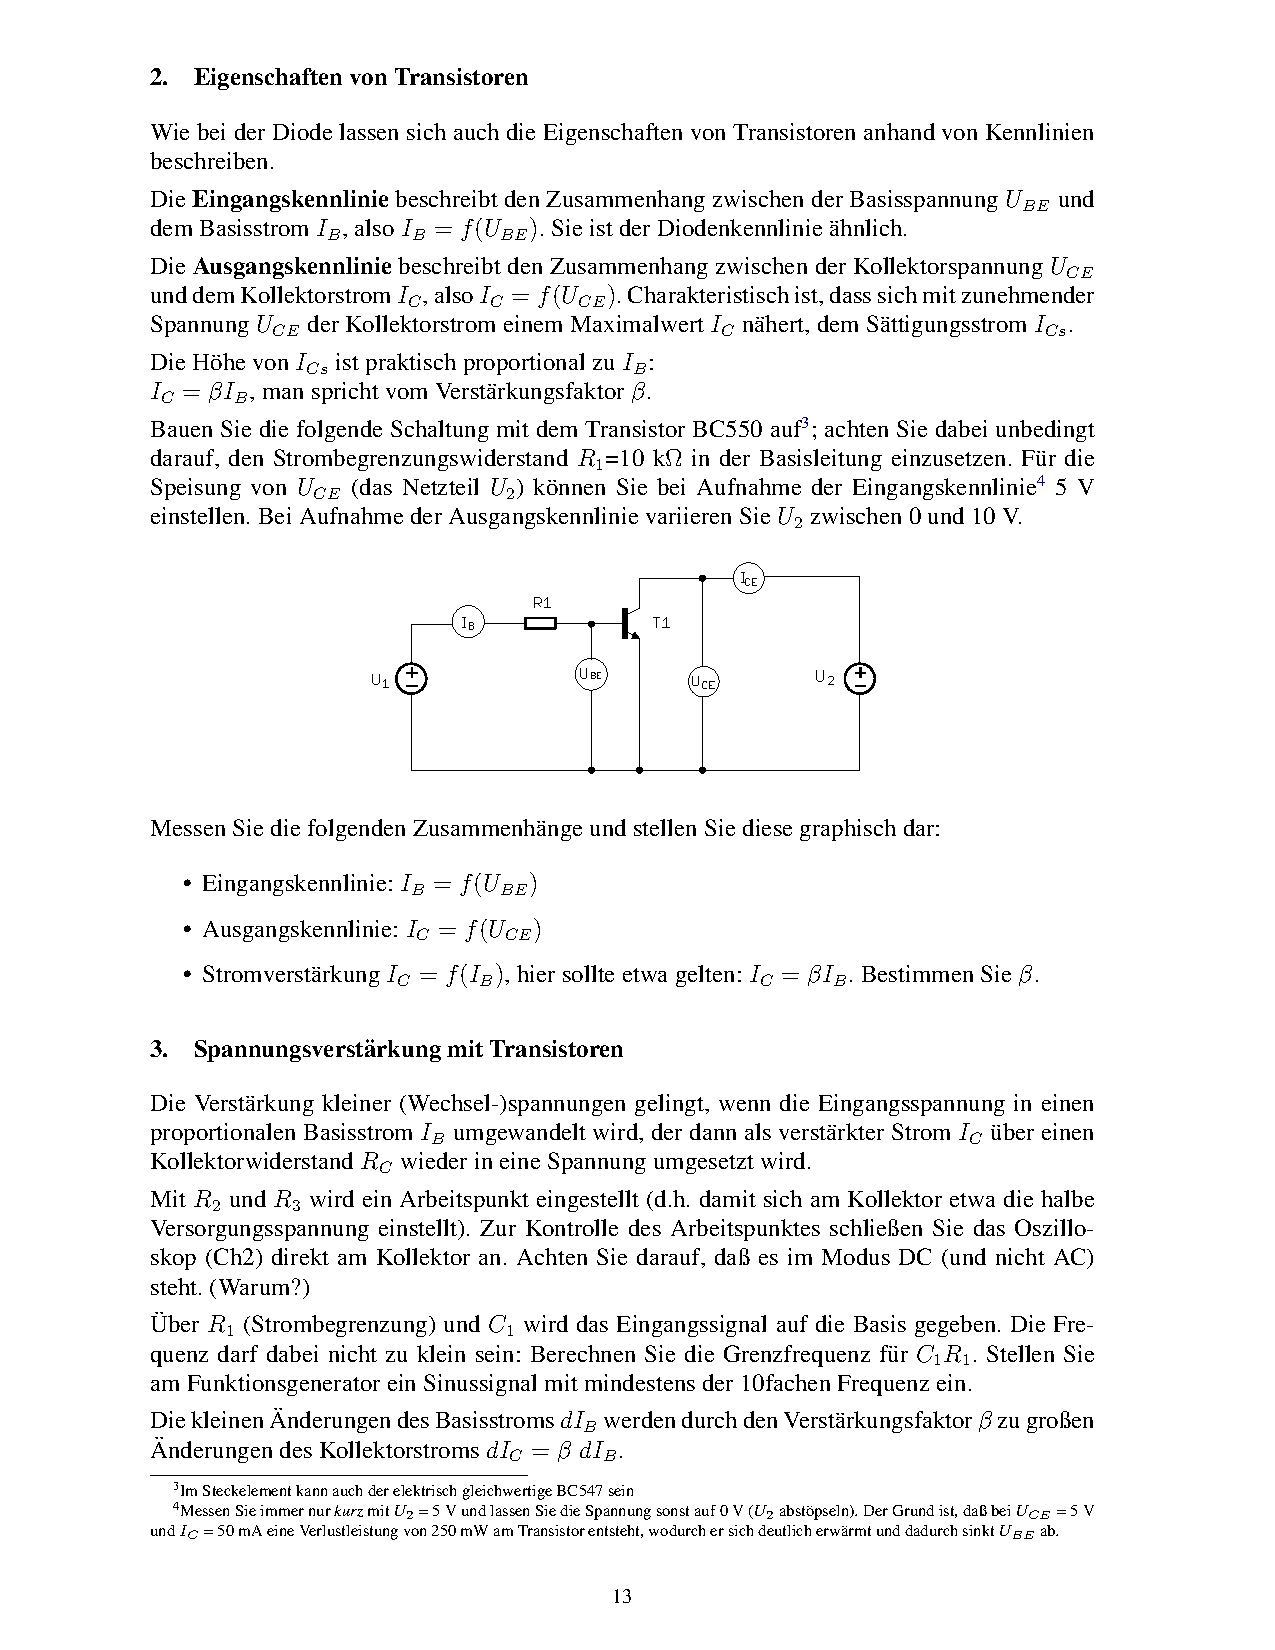
\includegraphics[trim = 10mm 145mm 10mm 90mm, clip, scale = 1]{ep3_14[Page13].pdf}
  	\caption[Schaltskizze für die Messung der Ein- und Ausgangskennlinie eines Transistors]{Schaltskizze für die Messung der Ein- und Ausgangskennlinie eines Transistors\footnotemark}
  \label{fig:1}
\end{figure}
\footnotetext{Abbildung entnommen von http://www.atlas.uni-wuppertal.de/$\sim$kind/ep3\_14.pdf Seite 13 am 10.11.2014}

\subsection{Versuchsdurchführung}
%erklären, !was! wir machen, !warum! wir das machen und mit welchem ziel
%(wichtig) präzize erklären, wie bei dem versuch vorgegangen und was gemacht wurde
Zuerst soll die Eingangskennlinie  $I_B$ gegen $U_{BE}$ aufgenommen werden. Zu erwarten ist ein diodenähnlicher exponentieller Zusammenhang, wobei die Spannung $U_{CE}$  bei dieser Messung auf \unit[5]{V} gestellt wird ($I_B = f(U_{BE})$). Danach wird die Ausgangskennlinie $I_C$ gegen $U_{CE}$ aufgenommen.
Anschließend soll die Stromverstärkung $\beta$ zwischen $I_B$ und $I_C$ bestimmt werden ($I_C = f(I_B)$). Es muss dabei beachtet werden, dass die Spannung $U_{BE}$ kleiner als die Spannung $U_{CE}$ bleibt, da $I_C$ nur für relativ kleine Ströme $I_B$ linear von $I_B$ abhängt.
\subsection{Messergebnisse}
%die messwerte in !übersichtlichen! tabellen angegeben
%zu viele kleine tabellen in große tabellen überführen!
%zu große tabellen mit dem [scale]-befehl scalieren oder (falls zu lang) in zwei kleinere tabellen aufteilen
%(wichtig) vor !jeder! tabelle sagen, was gemessen wurde und wie die fehler gewählt wurden und ausreichend !erklären!, !warum! wir unsere fehler grade so gewählt haben

Die Fehler wurden mit dem angegebenem Fehler und der Ableseungenauigkeit bestimmt, dabei ergab sich für I$_\text{B}$ ein Fehler von 0,006mA und für U$_\text{BE}$ ein Fehler von 0,006V.

\begin{table}[H]
\caption{Daten aus der Messung der Eingangslinie}
\begin{center}
\begin{tabular}{|r|r|}
\hline
\multicolumn{1}{|l|}{I$_\text{B}$/mA} & \multicolumn{1}{l|}{U$_\text{BE}$/V} \\ \hline
0 & 0 \\ \hline
0 & 0,1 \\ \hline
0 & 0,21 \\ \hline
0 & 0,31 \\ \hline
0 & 0,42 \\ \hline
0 & 0,53 \\ \hline
0,01 & 0,62 \\ \hline
0,04 & 0,65 \\ \hline
0,08 & 0,66 \\ \hline
0,12 & 0,67 \\ \hline
0,16 & 0,673 \\ \hline
0,22 & 0,676 \\ \hline
0,32 & 0,679 \\ \hline
0,38 & 0,68 \\ \hline
0,4 & 0,685 \\ \hline
\end{tabular}
\end{center}
\label{tab:a_1_e}
\end{table}

Die Fehler wurden mit dem angegebenem Fehler und der Ableseungenauigkeit bestimmt, dabei ergab sich für I$_\text{CE}$ ein Fehler von 0,006mA und für U$_\text{CE}$ ein Fehler von 0,06V.

\begin{table}[H]
\caption{Daten aus der Messung der Ausgangslinie}
\begin{center}
\begin{tabular}{|r|r|}
\hline
\multicolumn{1}{|l|}{I$_\text{CE}$/mA} & \multicolumn{1}{l|}{U$_\text{CE}$/V} \\ \hline
0 & 0 \\ \hline
7,9 & 0,4 \\ \hline
8 & 0,8 \\ \hline
8 & 1,9 \\ \hline
8,1 & 2,9 \\ \hline
8,3 & 3,8 \\ \hline
8,4 & 4,9 \\ \hline
8,7 & 5,9 \\ \hline
8,8 & 6,8 \\ \hline
9 & 7,9 \\ \hline
9,3 & 8,8 \\ \hline
9,6 & 9,8 \\ \hline
\end{tabular}
\end{center}
\label{tab:a_1_a}
\end{table}


Die Fehler wurden mit dem angegebenem Fehler und der Ableseungenauigkeit bestimmt, dabei ergab sich für I$_\text{CE}$ ein Fehler von 0,06mA und für I$_\text{B}$ ein Fehler von 0,006V.


\begin{table}[H]
\caption{Daten aus der Messung der Verstärkung}
\begin{center}
\begin{tabular}{|r|r|}
\hline
\multicolumn{1}{|l|}{I$_\text{B}$/mA} & \multicolumn{1}{l|}{I$_\text{CE}$/mA} \\ \hline
0,035 & 8,6 \\ \hline
0,08 & 18,4 \\ \hline
0,124 & 26,1 \\ \hline
0,173 & 31,9 \\ \hline
0,225 & 36,5 \\ \hline
\end{tabular}
\end{center}
\label{tab:a_1_v}
\end{table}


\subsection{Auswertung}
%zuerst !alle! errechneten werte entweder in ganzen sätzen aufzählen, oder in tabellen (übersichtlicher) dargestellen, sowie auf die verwendeten formeln verweisen (die referenzierung der formel kann in der überschrift stehen)
%kurz erwähnen (vor der tabelle), warum wir das ganze ausrechnen bzw. was wir dort ausrechnen
%danach histogramme und plots erstellen, wobei wenn möglich funktionen durch die plots gelegt werden (zur not können auch splines benutzt werden, was aber angegeben werden muss)
%bei fits immer die funktion und das reduzierte chiquadrat mit angegeben, wobei auf verständlichkeit beim entziffern der zehnerpotenzen geachtet werden muss z.b. f(x)=(wert+-fehler)\cdot10^{irgendeine zahl}\cdot x + (wert+-fehler)\cdot10^{irgendeine zahl}
%bei jedem fit erklären, nach welchem zusammenhang gefittet wurde und warum!
%bei plots darauf achten, dass die achsenbeschriftung (auch die tics) die richtige größe haben und die legende im plot nicht die messwerte verdeckt
%kurz die aufgabenstellung abgehandeln
%2-----------------------------------------------2

Graphisch dargestellt ergibt sich für die Eingangslinie Abbildung \ref{fig:a_e}.

\begin{figure}[H] 
  \centering
    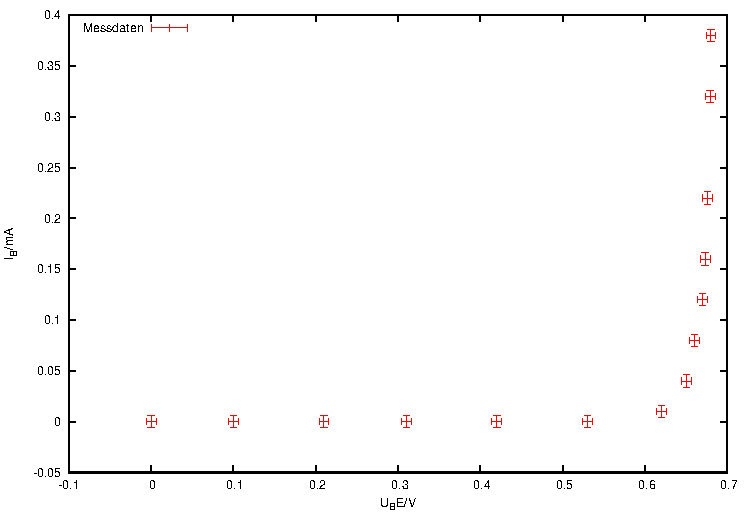
\includegraphics[scale = 0.7]{a_e.pdf}
  	\caption[Eingangslinie des Transistors]{Eingangslinie des Transistors}
  \label{fig:a_e}
\end{figure}

Plottet man die Daten aus der Messung der Ausgangslinie erhält man den Plot in Abbildung \ref{fig:a_a}.

\begin{figure}[H] 
  \centering
    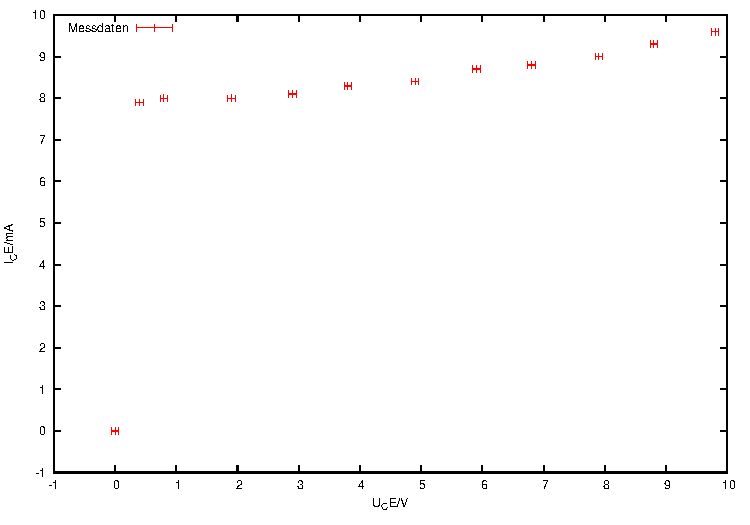
\includegraphics[scale = 0.7]{a_a.pdf}
  	\caption[Ausgangslinie des Transistors]{Ausgangslinie des Transistors}
  \label{fig:a_a}
\end{figure}

Zur Bestimmung der Verstärkung wurden die I$_\text{B}$ und I$_\text{CE}$ gegeneinander aufgetragen und die Messdaten mit der Funktion f(x)=m$\cdot$x+b gefittet, dabei sind m und b die freien Parameter. Durch den Fit ergab sich dann f(x)=(145.595$\pm$15.57)$\cdot$x+(5.75121$\pm$2.24). Die Verstärkung liegt bei 145.595$\pm$15.57.

\begin{figure}[H] 
  \centering
    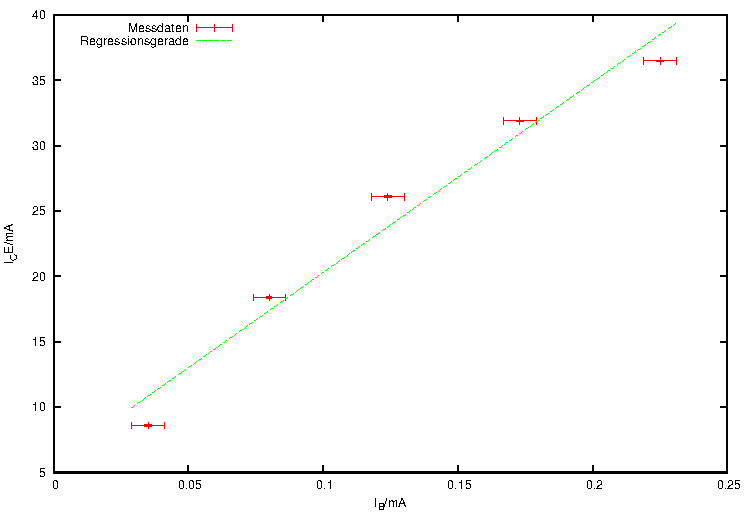
\includegraphics[scale = 0.7]{a_v.pdf}
  	\caption[Messung von I$_\text{CE}$ in Abhängigkeit von I$_\text{B}$]{Messung von I$_\text{CE}$ in Abhängigkeit von I$_\text{B}$}
  \label{fig:a_v}
\end{figure}

\subsection{Diskussion}
%(immer) die gemessenen werte und die bestimmten werte über die messfehler mit literaturwerten oder untereinander vergleichen
%in welchem fehlerintervall des messwertes liegt der literaturwert oder der vergleichswert?
%wie ist der relative anteil des fehlers am messwert und damit die qualität unserer messung?
%in einem satz erklären, wie gut unser fehler und damit unsere messung ist
%kurz erläutern, wie systematische fehler unsere messung beeinflusst haben könnten
%(wichtig) zum schluss ansprechen, in wie weit die ergebnisse mit der theoretischen vorhersage übereinstimmen
%--------------------------------------------------------------------------------------------
%falls tabellen mit den messwerten zu lang werden, kann die section mit den messwerten auch hinter der diskussion angefügt bzw. eine section mit dem anhang eingefügt werden.
%1-----------------------------------------------1

Die aufgenommenen Eingangs- und Ausgangslinien entsprechen den Theoretischen Linien wie sie in der Praktikumsanleitung auf Seite 5 angegeben sind. Für die Verstärkung wurde in der Praktikumsanleitung auf Seite 5 ein Wertebereich von 200 bis 500 angegeben, der von uns bestimmte Wert liegt bei 145.595$\pm$15.57. Dies kommt zu einen von einer zu geringen Spannung U0 mit 5V, welche für bessere Messergebnisse größer hätte sein sollten. Zum anderen an deren, an der Größe der Messwerte.

\section{Spannungsverstärkung mit Transistoren}
%kurz das ziel dieses versuchsteiles ansprechen, damit keine zwei überschriften direkt übereinander stehen!
%bei schwierigeren versuchen kann auch der theoretische hintergrund erläutert werden. (mit formeln, herleitungen und erklärungen)
Ziel dieses Versuches ist die Verstärkung kleiner Wechselspannungen mithilfe des Transistors.
\subsection{Verwendete Materialien}
%(immer) eine skizze oder ein foto einfügen, die geräte/materialien !nummerieren! und z.b. eine legende dazu schreiben, besser wäre es das ganze in einem Fließtext gut zu beschreiben.
%falls am anfang des versuches nicht klar ist, was alles verwendet wird, wenn möglich erst am ende ein großes foto von den verwendeten materialien machen!\\

Im Versuch wurde ein Funktionsgenerator als Spannungsquelle verwendet, mehrere Widerstände, ein Transistor, ein Potentiometer und zwei DMMs.

\subsection{Versuchsaufbau}
%skizze zum versuchsaufbau (oder foto) einfügen,   es muss erklärt werden wie das ganze funktioniert und welche speziellen einstellungen verwendet wurden (z.b. welche knöpfe an den geräten für die messung verdreht wurden)

\begin{itemize}
\item	T1 BC550

\item	C1 100nF

\item	R1 1k$\Omega$

\item	R2 100k$\Omega$

\item	R3 10k$\Omega$

\item	R4 1k$\Omega$ oder 10k$\Omega$

\item	C2 1$\mu$F

\item	Versorgungsspannung 10V
\end{itemize}

\begin{figure}[H] 
  \centering
    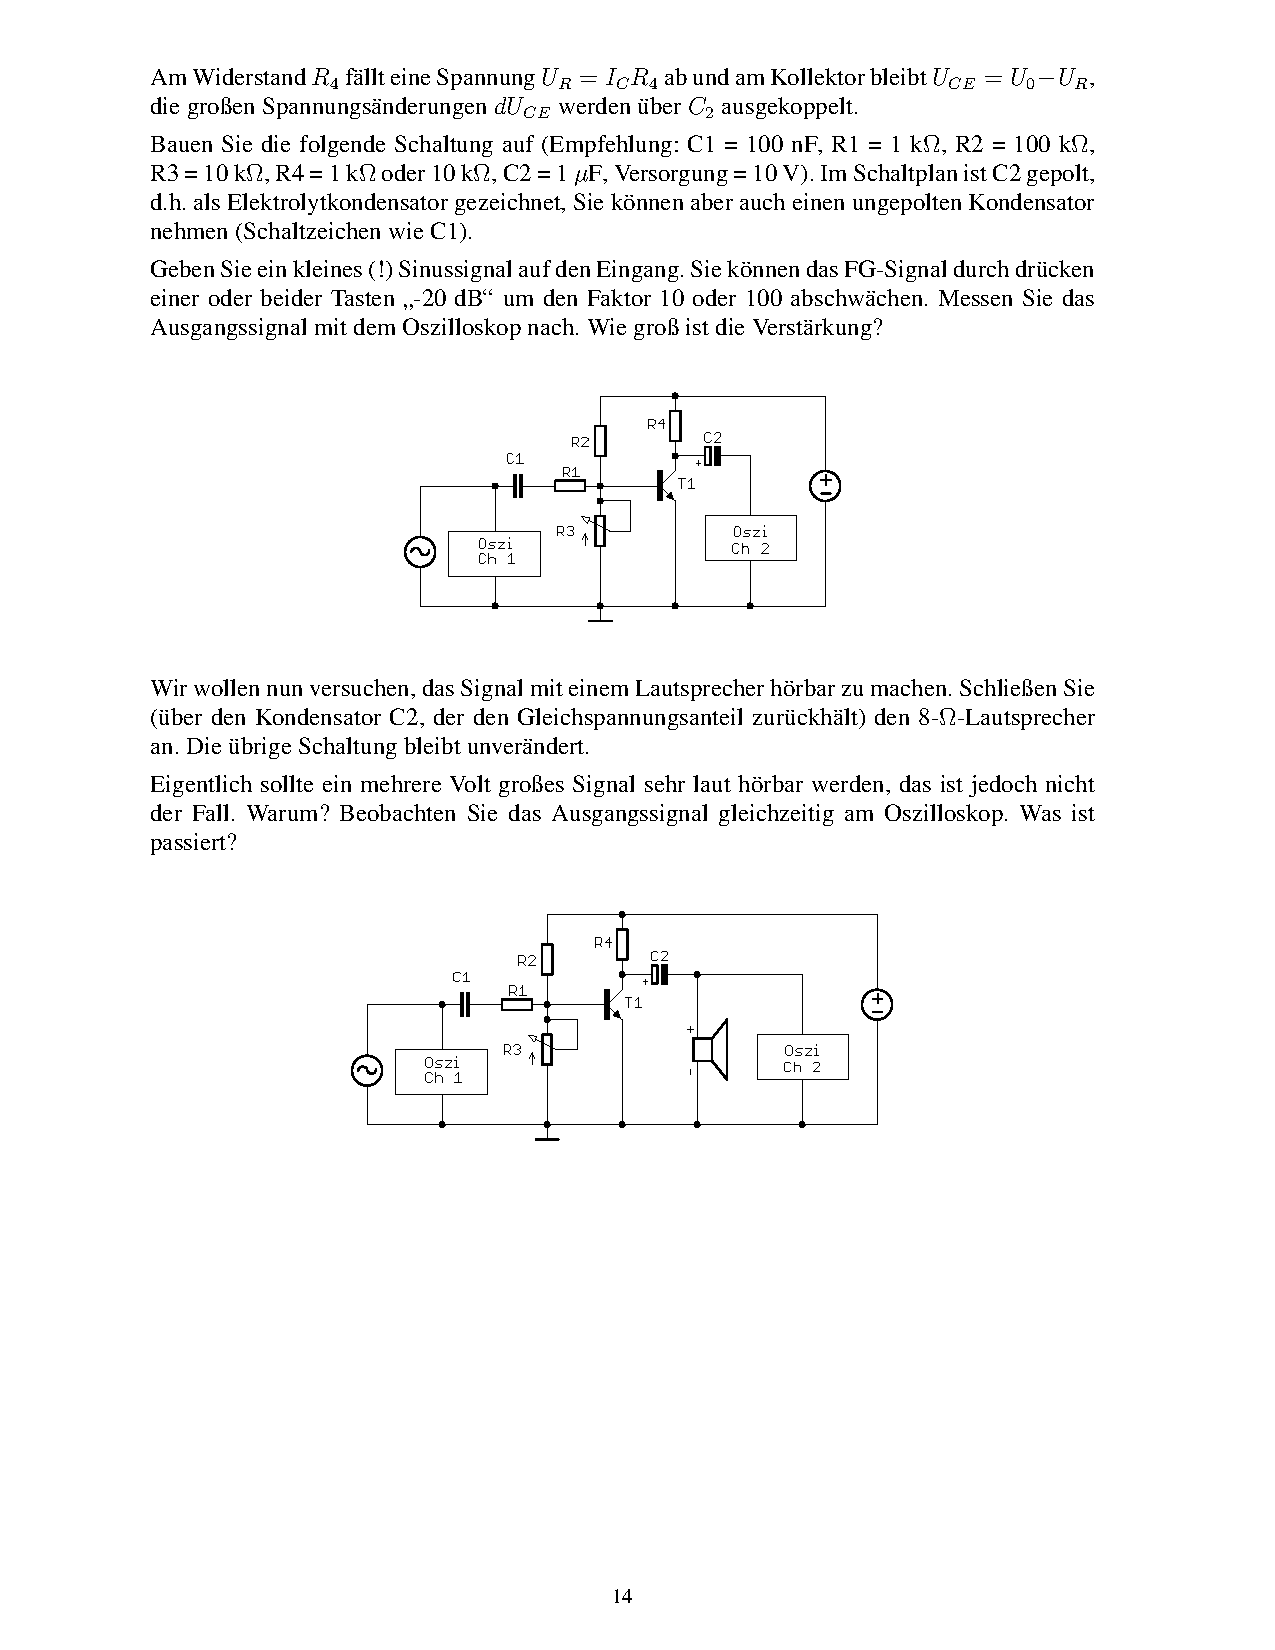
\includegraphics[trim = 10mm 165mm 10mm 60mm, clip, scale = 1]{ep3_14[Page14].pdf}
  	\caption[Schaltskizze für die Messung des Spannungsverstärkungsfaktors]{Schaltskizze für die Messung des Spannungsverstärkungsfaktors\footnotemark}
  \label{fig:2}
\end{figure}
\footnotetext{Abbildung entnommen von http://www.atlas.uni-wuppertal.de/$\sim$kind/ep3\_14.pdf Seite 14 am 10.11.2014}


\begin{itemize}
\item	T1 BC550

\item	C1 100nF

\item	R1 1k$\Omega$

\item	R2 100k$\Omega$

\item	R3 10k$\Omega$

\item	R4 1k$\Omega$ oder 10k$\Omega$

\item	C2 1$\mu$F

\item	Versorgungsspannung 10V

\item	8$\Omega$ Lautsprecher
\end{itemize}

\begin{figure}[H] 
  \centering
    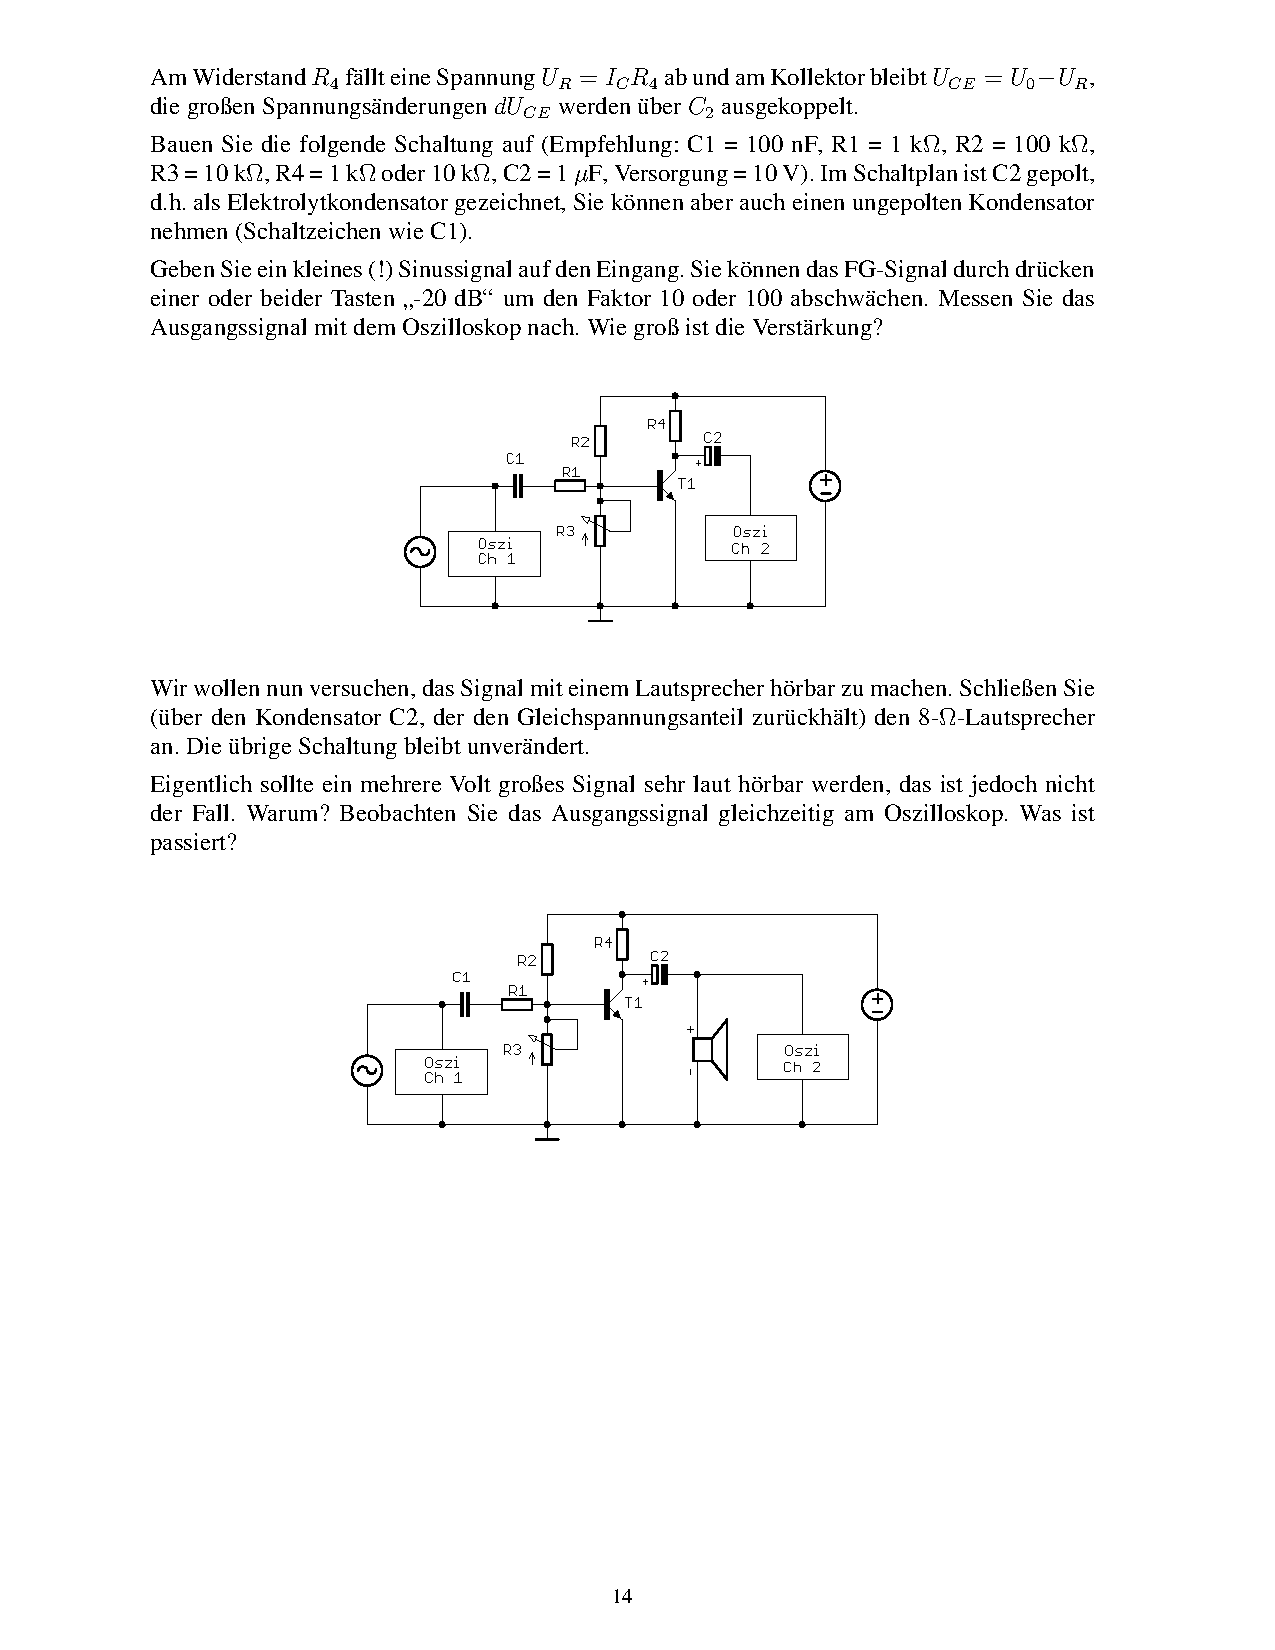
\includegraphics[trim = 10mm 65mm 10mm 150mm, clip, scale = 1]{ep3_14[Page14].pdf}
  	\caption[Schaltskizze für die Messung des Spannungsverstärkungsfaktors und Audioausgabe des verstärkten Signals]{Schaltskizze für die Messung des Spannungsverstärkungsfaktors und Audioausgabe des verstärkten Signals\footnotemark}
  \label{fig:3}
\end{figure}
\footnotetext{Abbildung entnommen von http://www.atlas.uni-wuppertal.de/$\sim$kind/ep3\_14.pdf Seite 14 am 10.11.2014}

\subsection{Versuchsdurchführung}
%erklären, !was! wir machen, !warum! wir das machen und mit welchem ziel
%(wichtig) präzize erklären, wie bei dem versuch vorgegangen und was gemacht wurde
Mit dem Oszilloskop werden Ausgangs- und Eingangssignal bei der Schaltung für die Spannungsverstärkung aufgenommen, um den Verstärkungsfaktor zwischen Ausgangs und Eingangsspannung zu bestimmen. Im zweiten Teil soll ein Lautsprecher über den Kondensator angeschlossen werden. Da der Strom nur auf wenige Milliampere beschränkt ist, ist zu erwarten, dass die Spannung durch den extremen Spannungsteiler von $\frac{8}{1000 + 8}$ am Lautsprecher zusammenbricht und damit etwas zu hören ist.
\subsection{Auswertung}
%zuerst !alle! errechneten werte entweder in ganzen sätzen aufzählen, oder in tabellen (übersichtlicher) dargestellen, sowie auf die verwendeten formeln verweisen (die referenzierung der formel kann in der überschrift stehen)
%kurz erwähnen (vor der tabelle), warum wir das ganze ausrechnen bzw. was wir dort ausrechnen
%danach histogramme und plots erstellen, wobei wenn möglich funktionen durch die plots gelegt werden (zur not können auch splines benutzt werden, was aber angegeben werden muss)
%bei fits immer die funktion und das reduzierte chiquadrat mit angegeben, wobei auf verständlichkeit beim entziffern der zehnerpotenzen geachtet werden muss z.b. f(x)=(wert+-fehler)\cdot10^{irgendeine zahl}\cdot x + (wert+-fehler)\cdot10^{irgendeine zahl}
%bei jedem fit erklären, nach welchem zusammenhang gefittet wurde und warum!
%bei plots darauf achten, dass die achsenbeschriftung (auch die tics) die richtige größe haben und die legende im plot nicht die messwerte verdeckt
%kurz die aufgabenstellung abgehandeln
%2-----------------------------------------------2

Betrachtet man die Eingangsspannung und die Ausgangsspannung, siehe Abbildung \ref{fig:a_2_1}, so kann aus dem Verhältnis der Amplituden die Verstärkung bestimmt werden. Die Verstärkung ergibt sich mit 100.

\begin{figure}[H] 
  \centering
    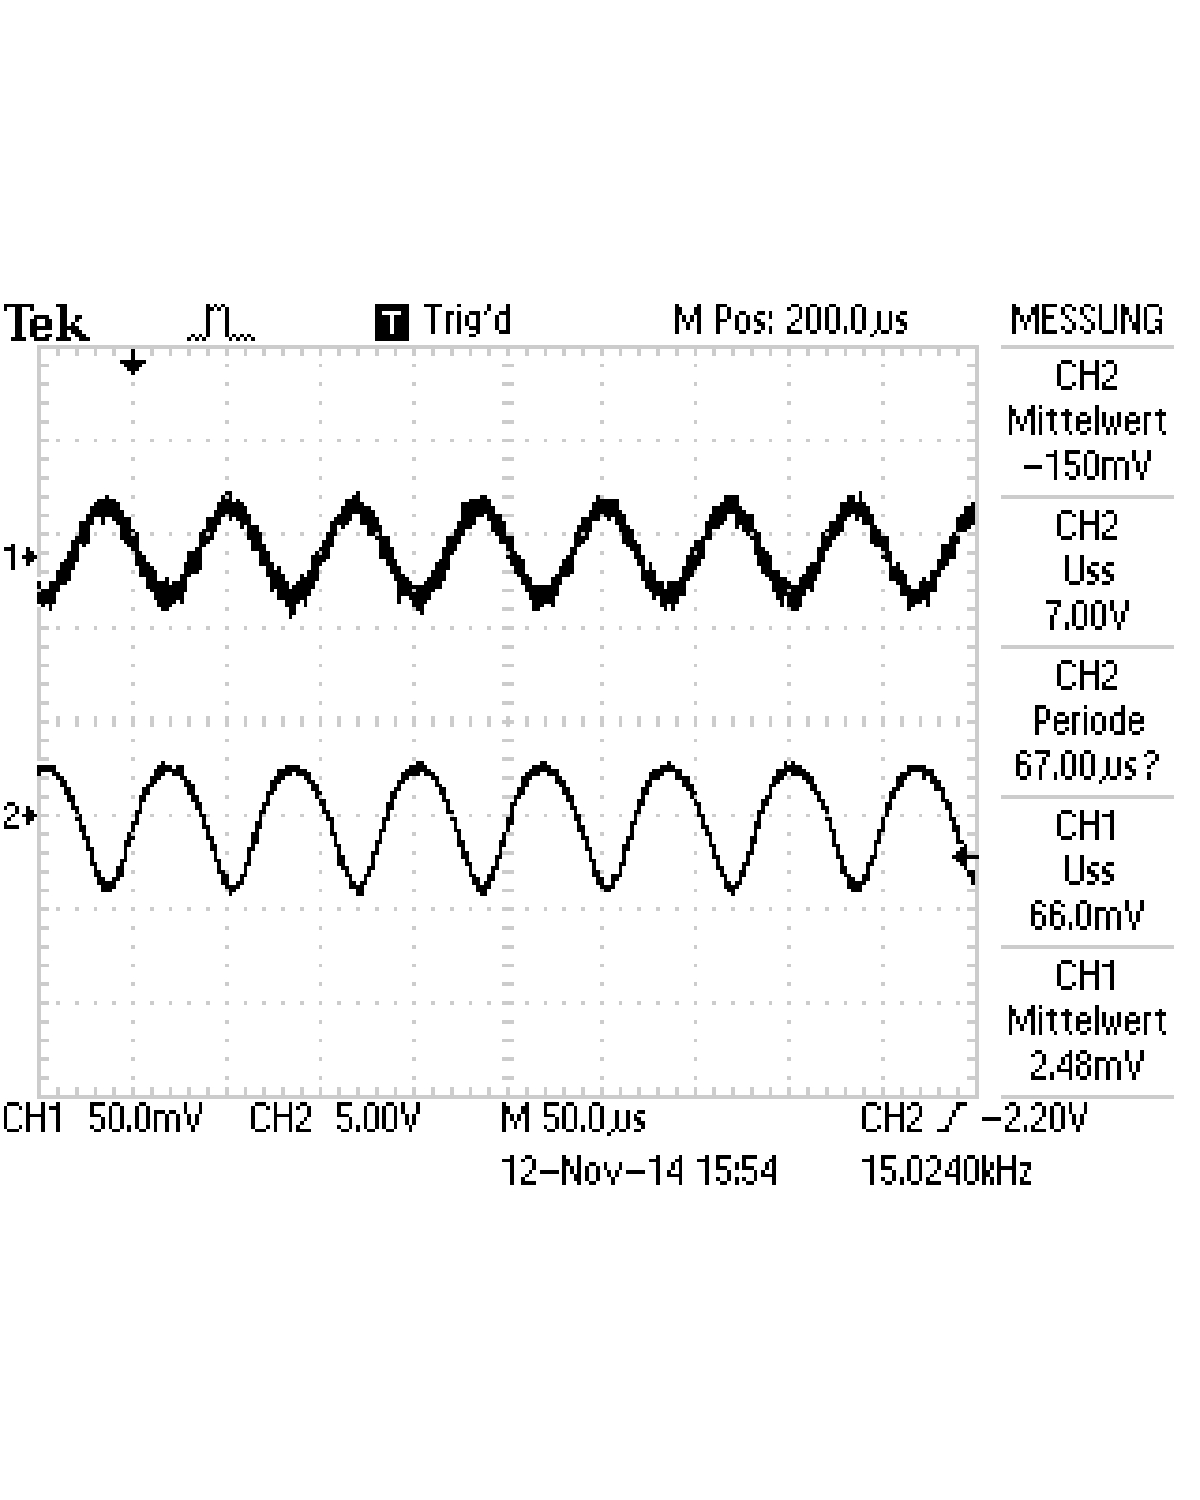
\includegraphics[scale = 0.7]{a_2_1.pdf}
  	\caption[Eingangsspannung und Ausgangsspannung, auf dem Oszilloskop]{Eingangsspannung und Ausgangsspannung, auf dem Oszilloskop}
  \label{fig:a_2_1}
\end{figure}

Schließt man nun den Lautsprecher an, so ergibt sich für die Eingangsspannung und die Ausgangsspannung auf dem Oszilloskop der Verlauf in Abbildung \ref{fig:a_2_2}. Der Spannungsteiler von $\frac{8}{1000 + 8}$ bewirkt nur eine sehr kleine Spannung am Lautsprecher, wodurch kein Signal ausgegeben wird.


\begin{figure}[H] 
  \centering
    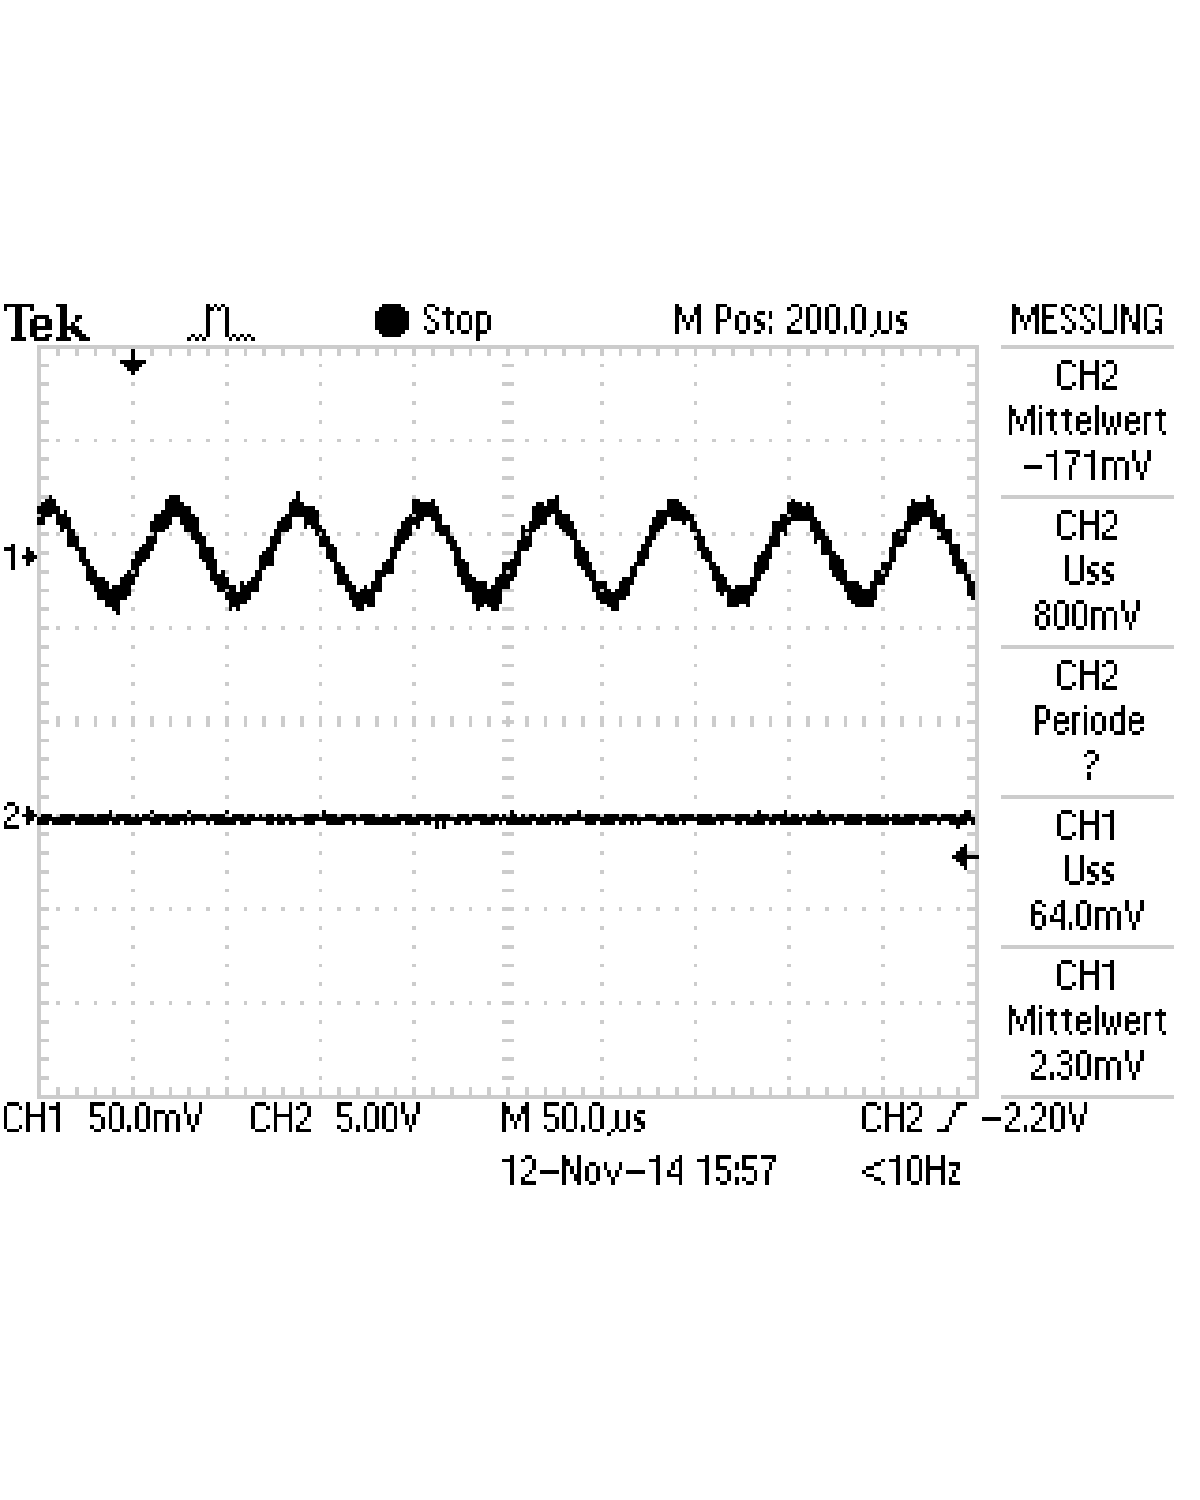
\includegraphics[scale = 0.7]{a_2_2.pdf}
  	\caption[Eingangsspannung und Ausgangsspannung, auf dem Oszilloskop, mit Lautsprecher]{Eingangsspannung und Ausgangsspannung, auf dem Oszilloskop, mit Lautsprecher}
  \label{fig:a_2_2}
\end{figure}

\subsection{Diskussion}
%(immer) die gemessenen werte und die bestimmten werte über die messfehler mit literaturwerten oder untereinander vergleichen
%in welchem fehlerintervall des messwertes liegt der literaturwert oder der vergleichswert?
%wie ist der relative anteil des fehlers am messwert und damit die qualität unserer messung?
%in einem satz erklären, wie gut unser fehler und damit unsere messung ist
%kurz erläutern, wie systematische fehler unsere messung beeinflusst haben könnten
%(wichtig) zum schluss ansprechen, in wie weit die ergebnisse mit der theoretischen vorhersage übereinstimmen
%--------------------------------------------------------------------------------------------
%falls tabellen mit den messwerten zu lang werden, kann die section mit den messwerten auch hinter der diskussion angefügt bzw. eine section mit dem anhang eingefügt werden.
%1-----------------------------------------------1

Wie erwartet wurde eine Verstärkung im Bereich von 100 Gemessen und am Lautsprecher war kaum etwas zu hören, USS kann an der Graphik (Abb. \ref{fig:a_2_1}) abgelesen werden. 

\section{Stromverstärkung mit Transistoren}
%kurz das ziel dieses versuchsteiles ansprechen, damit keine zwei überschriften direkt übereinander stehen!
%bei schwierigeren versuchen kann auch der theoretische hintergrund erläutert werden. (mit formeln, herleitungen und erklärungen)
Neben der Spannungsverstärkung kann mit dem Transistor auch der Strom verstärkt werden, um höhere Ausgangsströme zu erreichen.
\subsection{Verwendete Geräte}
%(immer) eine skizze oder ein foto einfügen, die geräte/materialien !nummerieren! und z.b. eine legende dazu schreiben, besser wäre es das ganze in einem Fließtext gut zu beschreiben.
%falls am anfang des versuches nicht klar ist, was alles verwendet wird, wenn möglich erst am ende ein großes foto von den verwendeten materialien machen!\\
Als Spannungsquelle wird ein Funktionsgenerator verwendet, zur Strom- und Spannungsverstärkung werden ein BC550 und ein BD137 Transistor verwendet. Zudem wurden verscheiden Widerstände , Kondensatoren und Potentiometer verwendet. Zur Messung wurden DMMs oder ein Oszilloskop verwendet, sowie ein Lautsprecher zur Signalausgabe.


\subsection{Versuchsaufbau}
%skizze zum versuchsaufbau (oder foto) einfügen,   es muss erklärt werden wie das ganze funktioniert und welche speziellen einstellungen verwendet wurden (z.b. welche knöpfe an den geräten für die messung verdreht wurden)

\begin{itemize}
\item	T1 BD137

\item	R1 10k$\Omega$

\item	R2 1k$\Omega$

\item	R3 100$\Omega$

\item	Versorgungsspannung 10V

\end{itemize}

\begin{figure}[H] 
  \centering
    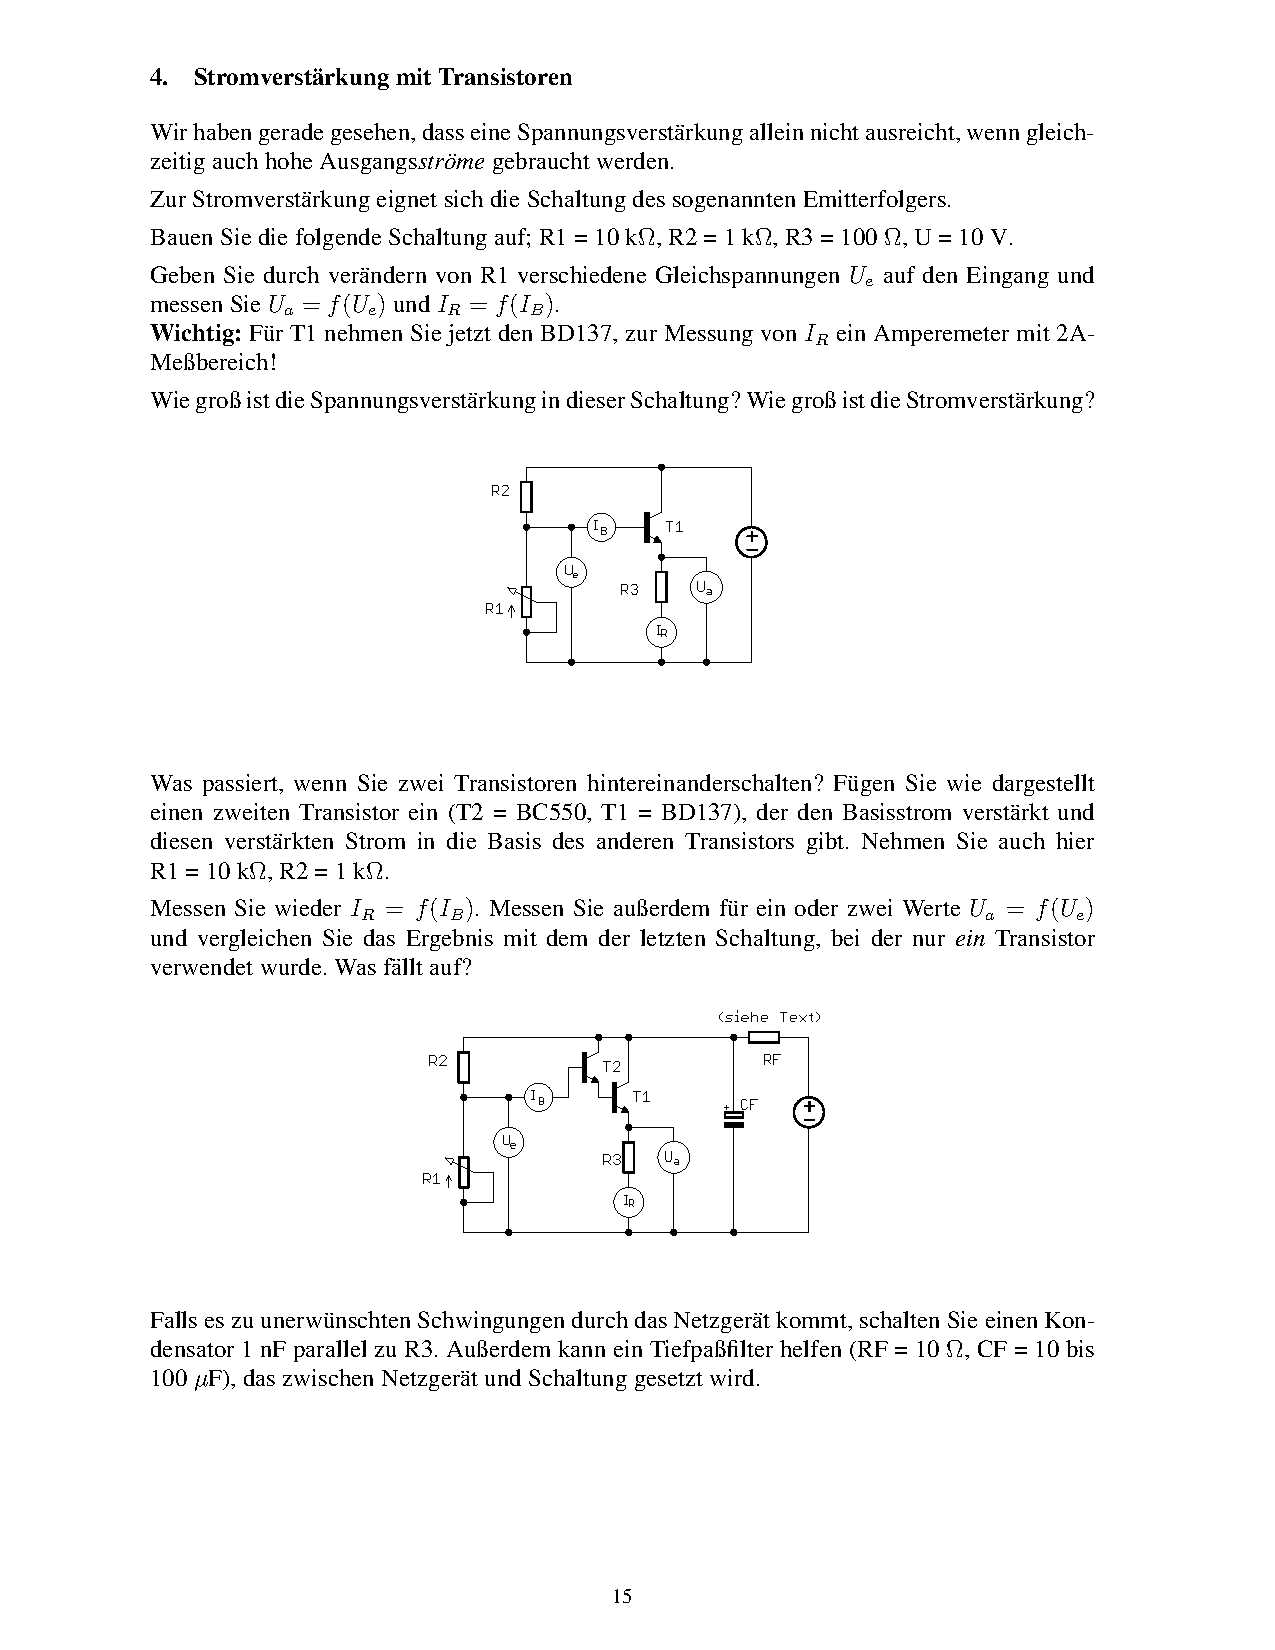
\includegraphics[trim = 10mm 165mm 10mm 75mm, clip, scale = 1]{ep3_14[Page15].pdf}
  	\caption[Schaltskizze für die Messung des Stromverstärkungsfaktors]{Schaltskizze für die Messung des Stromverstärkungsfaktors\footnotemark}
  \label{fig:4}
\end{figure}
\footnotetext{Abbildung entnommen von http://www.atlas.uni-wuppertal.de/$\sim$kind/ep3\_14.pdf Seite 15 am 10.11.2014}


\begin{itemize}
\item	T1 BD137

\item	T2 BC550

\item	R1 10k$\Omega$

\item	R2 1k$\Omega$

\item	R3 100$\Omega$

\item	Versorgungsspannung 10V

\item	CF 10-100$\mu$F

\end{itemize}

\begin{figure}[H] 
  \centering
    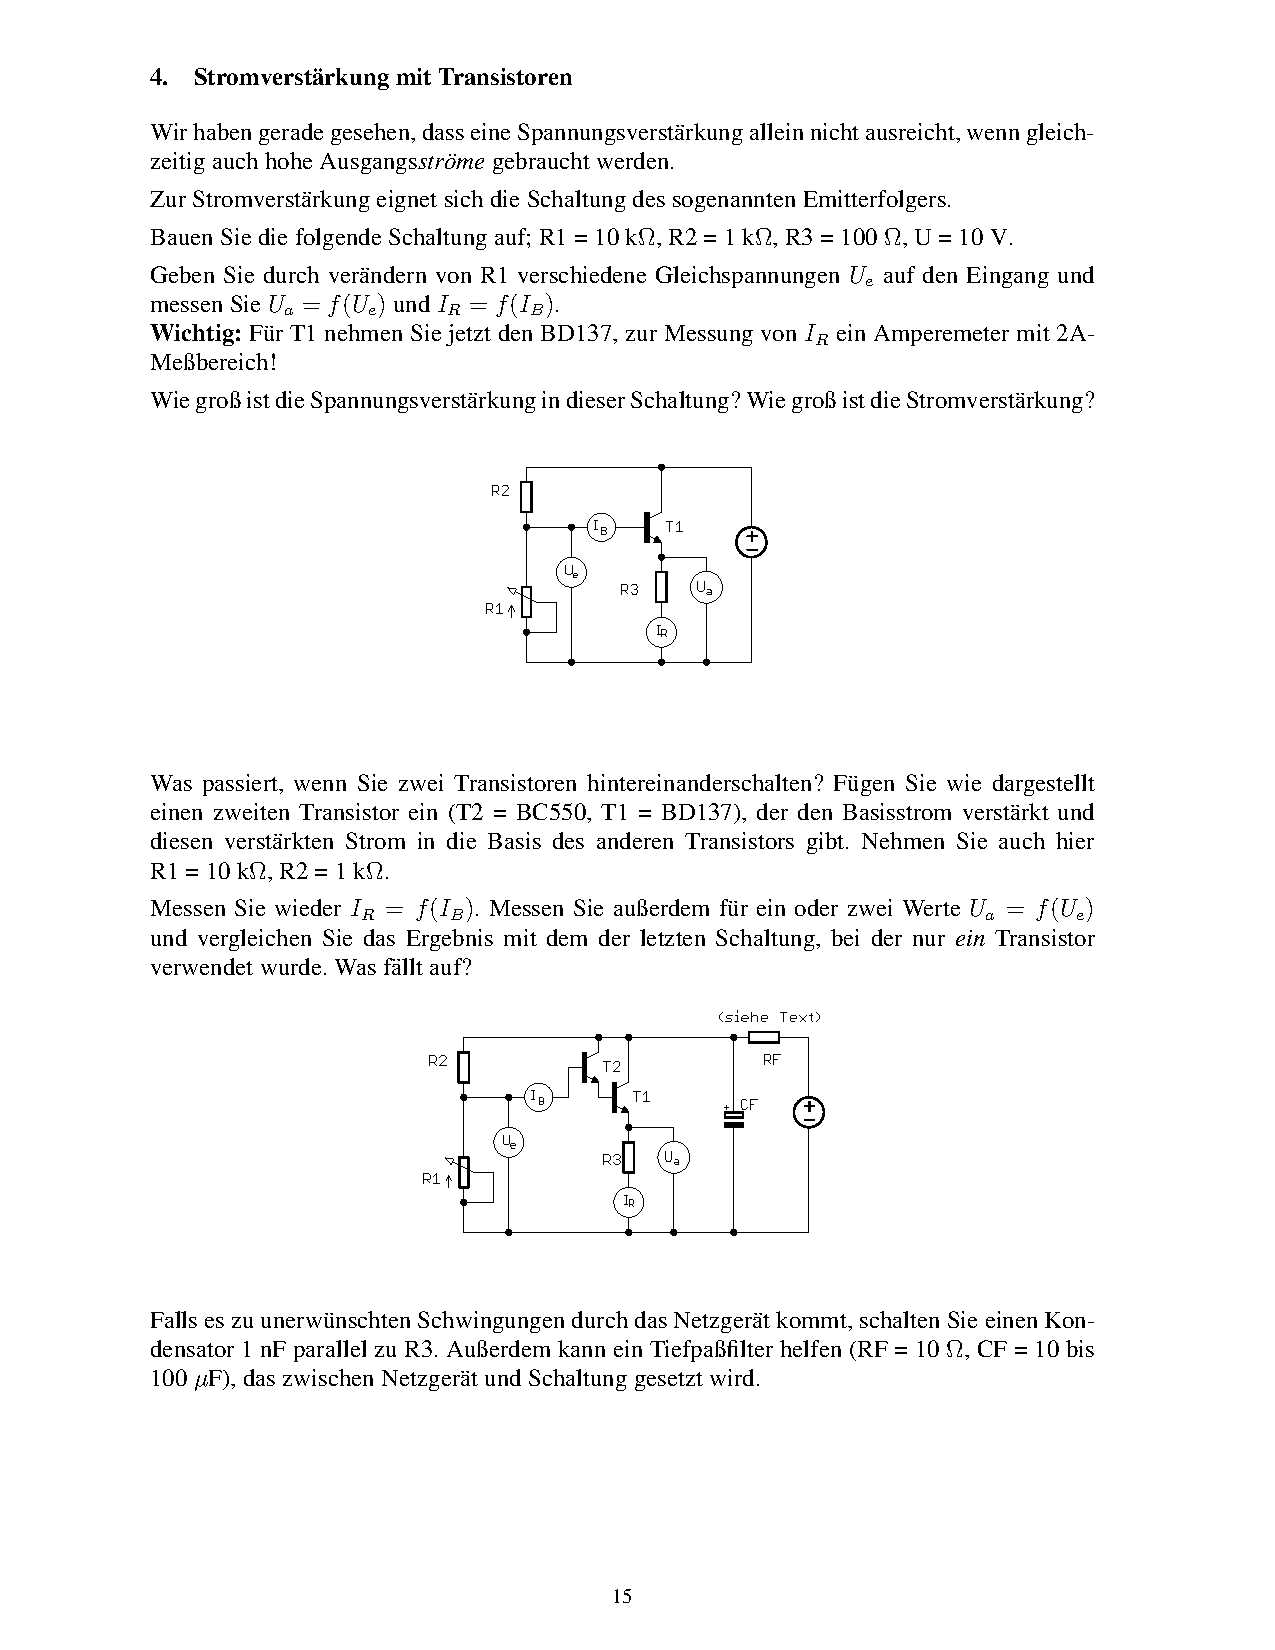
\includegraphics[trim = 10mm 65mm 10mm 174mm, clip, scale = 1]{ep3_14[Page15].pdf}
  	\caption[Schaltskizze für die Messung des Stromverstärkungsfaktors mit zwei hinter einander geschalteten Transistoren]{Schaltskizze für die Messung des Stromverstärkungsfaktors mit zwei hinter einander geschalteten Transistoren\footnotemark}
  \label{fig:5}
\end{figure}
\footnotetext{Abbildung entnommen von http://www.atlas.uni-wuppertal.de/$\sim$kind/ep3\_14.pdf Seite 15 am 10.11.2014}

\begin{itemize}
\item	T1 BD137

\item	T2 BC550

\item	C1 1$\mu$F

\item	R1 1k$\Omega$

\item	R2 100k$\Omega$

\item	R3 10k$\Omega$

\item	R4 1k$\Omega$

\item	R5 100$\Omega$

\item	R4 1k$\Omega$ oder 10k$\Omega$

\item	C2 100$\mu$F

\item	CF 10-100$\mu$F
\end{itemize}

\begin{figure}[H] 
  \centering
    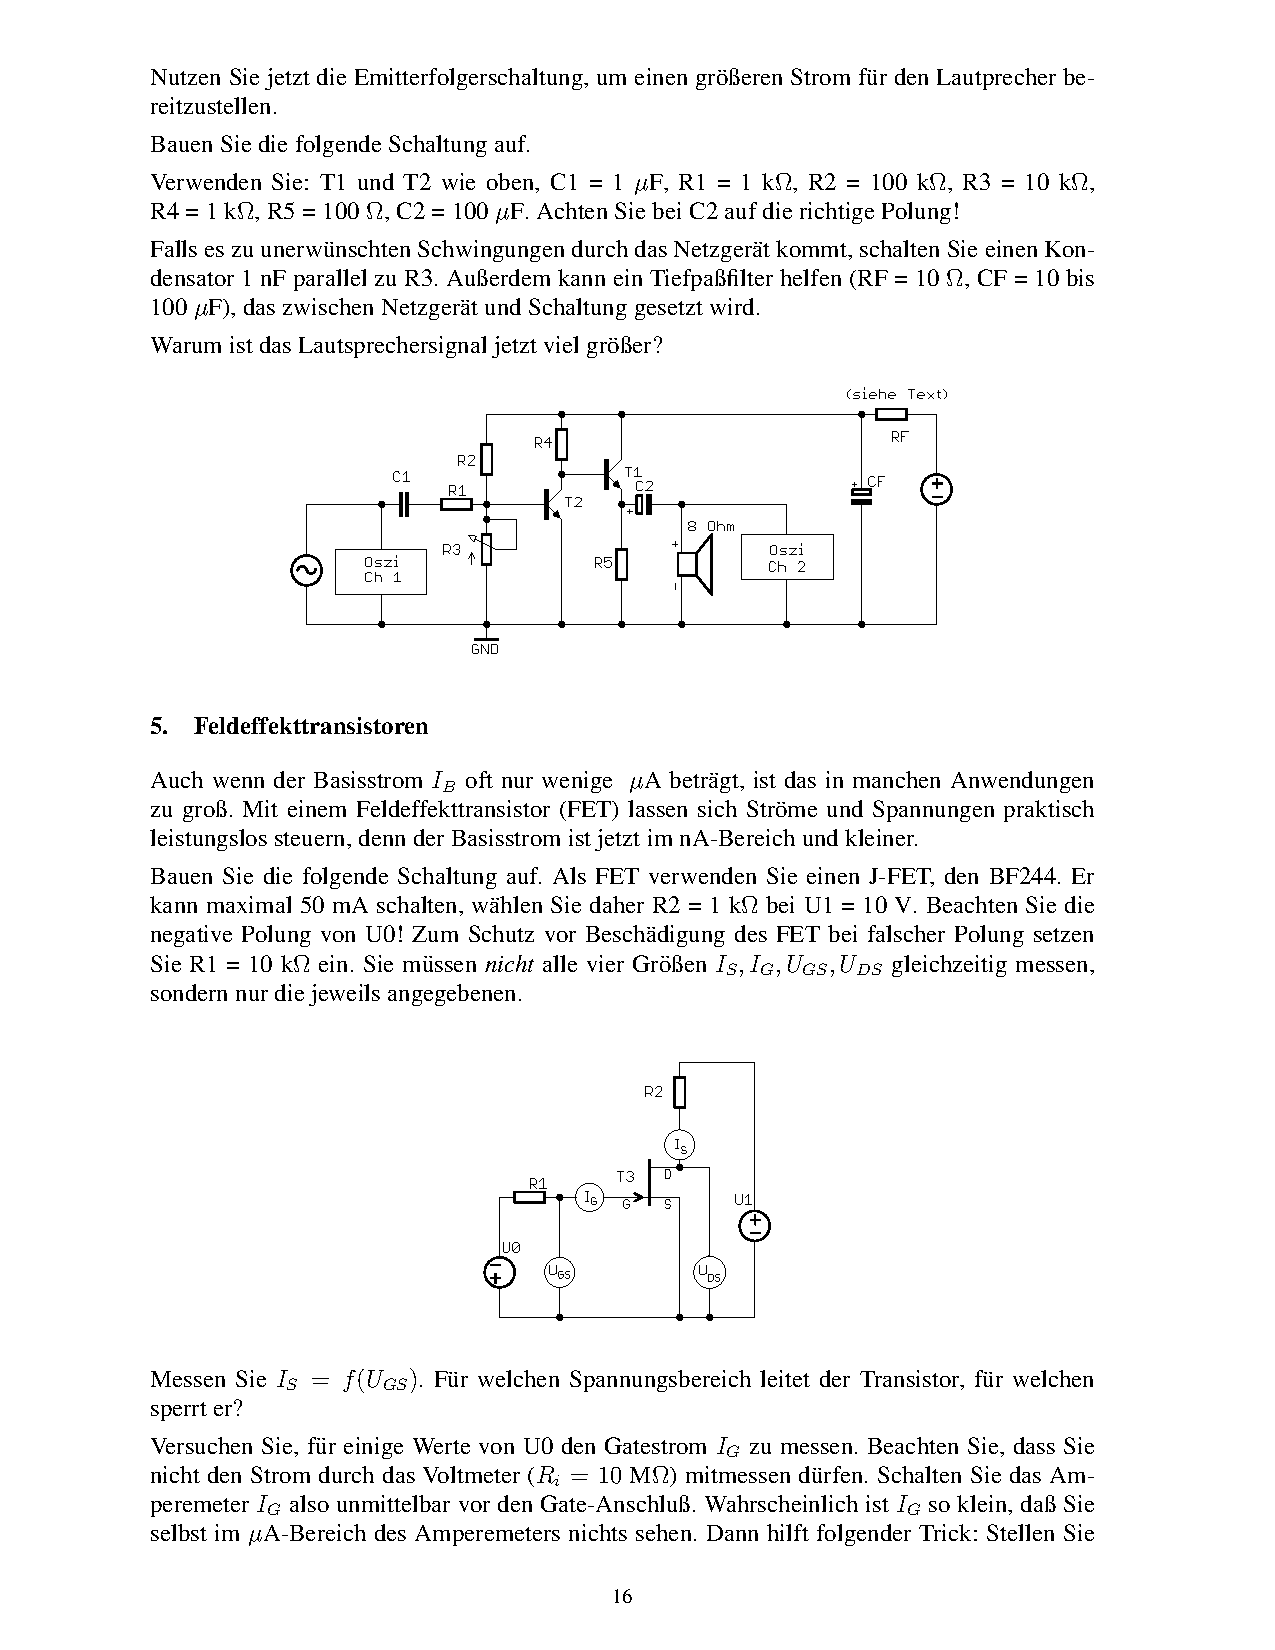
\includegraphics[trim = 10mm 165mm 10mm 69mm, clip, scale = 1]{ep3_14[Page16].pdf}
  	\caption[Schaltskizze für die Messung des Stromverstärkungsfaktors mit zwei hinter einander geschalteten Transistoren und Audioausgabe des verstärkten Signals]{Schaltskizze für die Messung des Stromverstärkungsfaktors mit zwei hinter einander geschalteten Transistoren und Audioausgabe des verstärkten Signals\footnotemark}
  \label{fig:6}
\end{figure}
\footnotetext{Abbildung entnommen von http://www.atlas.uni-wuppertal.de/$\sim$kind/ep3\_14.pdf Seite 16 am 10.11.2014}

\subsection{Versuchsdurchführung}
%erklären, !was! wir machen, !warum! wir das machen und mit welchem ziel
%(wichtig) präzize erklären, wie bei dem versuch vorgegangen und was gemacht wurde
Zur Stromverstärkung wird die Schaltung des sogenannten Emittierfolgers aufgebaut. Es soll $U_a = f(U_e)$ und $I_R = f(I_B)$ bestimmt werden. Als Verstärkungsfaktor wird, da $I_B \ll I_C$ ist, ebenfalls $\beta$ erwartet.
\subsection{Messergebnisse}
%die messwerte in !übersichtlichen! tabellen angegeben
%zu viele kleine tabellen in große tabellen überführen!
%zu große tabellen mit dem [scale]-befehl scalieren oder (falls zu lang) in zwei kleinere tabellen aufteilen
%(wichtig) vor !jeder! tabelle sagen, was gemessen wurde und wie die fehler gewählt wurden und ausreichend !erklären!, !warum! wir unsere fehler grade so gewählt haben

Die Fehler wurden mit dem angegeben Fehler und der Ableseungenauigkeit bestimmt, für U$_\text{A}$ und U$_\text{E}$ ergibt sich ein Fehler von 0,06V.

\begin{table}[H]
\caption{Daten aus der Messung der Ein- und Ausgangsspannung}
\begin{center}
\begin{tabular}{|r|r|}
\hline
\multicolumn{1}{|l|}{U$_\text{E}$/V} & \multicolumn{1}{l|}{U$_\text{A}$/V} \\ \hline
0 & 0 \\ \hline
0,49 & 0 \\ \hline
0,88 & 0,26 \\ \hline
1,32 & 0,68 \\ \hline
1,62 & 0,96 \\ \hline
2,05 & 1,38 \\ \hline
2,44 & 1,76 \\ \hline
2,77 & 2,09 \\ \hline
3,16 & 2,47 \\ \hline
3,56 & 2,87 \\ \hline
3,97 & 3,28 \\ \hline
\end{tabular}
\end{center}
\label{tab:a_3_u}
\end{table}

Die Fehler wurden mit dem angegeben Fehler und der Ableseungenauigkeit bestimmt, I$_\text{R}$ ergibt sich ein Fehler von 0,06mA und für I$_\text{B}$ ein Fehler von 0,0006mA.


\begin{table}[H]
\caption{Daten aus der Messung des Stromes I$_\text{R}$ und I$_\text{B}$}
\begin{center}
\begin{tabular}{|r|r|}
\hline
\multicolumn{1}{|l|}{I$_\text{R}$/mA} & \multicolumn{1}{l|}{I$_\text{B}$/mA} \\ \hline
0 & 0 \\ \hline
0,6 & 0,017 \\ \hline
1,1 & 0,026 \\ \hline
1,3 & 0,031 \\ \hline
1,8 & 0,04 \\ \hline
2,3 & 0,051 \\ \hline
2,7 & 0,057 \\ \hline
2,8 & 0,059 \\ \hline
\end{tabular}
\end{center}
\label{tab:a_3_i}
\end{table}


Die Fehler wurden mit dem angegeben Fehler und der Ableseungenauigkeit bestimmt, für U$_\text{A}$ und U$_\text{E}$ ergibt sich ein Fehler von 0,06V.

\begin{table}[H]
\caption{Daten aus der Messung der Spannungen U$_\text{E}$ udn U$_\text{A}$, mit zwei Transistoren}
\begin{center}
\begin{tabular}{|r|r|}
\hline
\multicolumn{1}{|l|}{U$_\text{E}$/V} & \multicolumn{1}{l|}{U$_\text{A}$/V} \\ \hline
1,84 & 0,61 \\ \hline
2,24 & 0,98 \\ \hline
\end{tabular}
\end{center}
\label{tab:a_3b_u}
\end{table}

Die Fehler wurden mit dem angegeben Fehler und der Ableseungenauigkeit bestimmt, I$_\text{R}$ ergibt sich ein Fehler von 0,006mA und für I$_\text{B}$ ein Fehler von 0,006nA.

\begin{table}[H]
\caption{Daten aus der Messung des Stromes  I$_\text{R}$ und I$_\text{B}$}
\begin{center}
\begin{tabular}{|r|r|}
\hline
\multicolumn{1}{|l|}{I$_\text{R}$/mA} & \multicolumn{1}{l|}{I$_\text{B}$/nA} \\ \hline
0,1 & 0,31 \\ \hline
0,2 & 0,42 \\ \hline
0,3 & 0,59 \\ \hline
0,5 & 0,71 \\ \hline
0,6 & 0,82 \\ \hline
0,7 & 0,91 \\ \hline
0,8 & 1,01 \\ \hline
\end{tabular}
\end{center}
\label{tab:a_3b_i}
\end{table}


\subsection{Auswertung}
%zuerst !alle! errechneten werte entweder in ganzen sätzen aufzählen, oder in tabellen (übersichtlicher) dargestellen, sowie auf die verwendeten formeln verweisen (die referenzierung der formel kann in der überschrift stehen)
%kurz erwähnen (vor der tabelle), warum wir das ganze ausrechnen bzw. was wir dort ausrechnen
%danach histogramme und plots erstellen, wobei wenn möglich funktionen durch die plots gelegt werden (zur not können auch splines benutzt werden, was aber angegeben werden muss)
%bei fits immer die funktion und das reduzierte chiquadrat mit angegeben, wobei auf verständlichkeit beim entziffern der zehnerpotenzen geachtet werden muss z.b. f(x)=(wert+-fehler)\cdot10^{irgendeine zahl}\cdot x + (wert+-fehler)\cdot10^{irgendeine zahl}
%bei jedem fit erklären, nach welchem zusammenhang gefittet wurde und warum!
%bei plots darauf achten, dass die achsenbeschriftung (auch die tics) die richtige größe haben und die legende im plot nicht die messwerte verdeckt
%kurz die aufgabenstellung abgehandeln
%2-----------------------------------------------2

Die Schaltung aus Abbildung \ref{fig:4} sollte auf die Eingenschaften der Strom- und Spannungsverstärkung untersuche werden. Dafür wurde die Ausgangsspannung in Abhängigkeit der Eingangsspannung gemessen, siehe Abbildung \ref{tab:a_3_u}. Zur Bestimmung der Stromverstärkung wurde I$_\text{R}$ in Abhängigkeit von I$_\text{B}$ gemessen, siehe Abbildung \ref{fig:a_3_i}.
Die Spannungsdifferenz zwischen Ausgangs- und Eingangsspannung ergab sich im Mittel mit 0,67V, was, wie erwartet, dem Arbeitspunkt des Transistors entspricht.

\begin{figure}[H] 
  \centering
    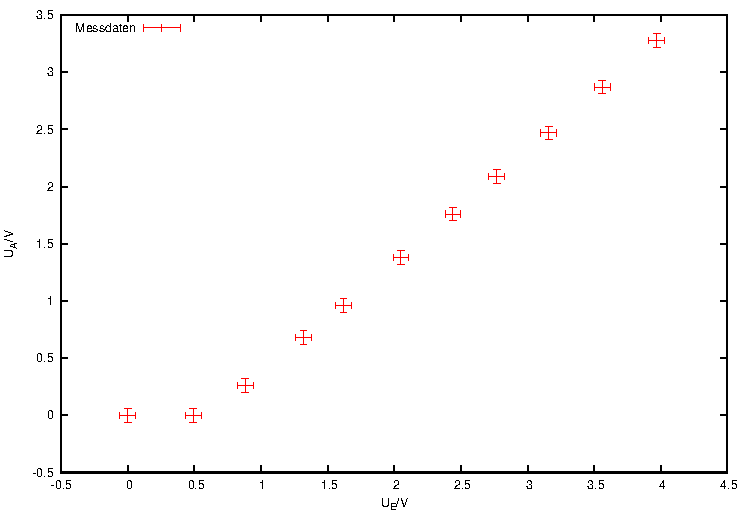
\includegraphics[scale = 0.7]{a_3_u.pdf}
  	\caption[Eingans- gegen Ausgangsspannung]{Eingans- gegen Ausgangsspannung}
  \label{fig:a_3_u}
\end{figure}

Die Stromverstärkung wurde durch das anfitten der Funktion f(x)=m$\cdot$x+b bestimmt. Dabei wurden die Parameter m und b gefittet. Durch den fit ergab sich f(x)=(47.74$\pm$1.77)$\cdot$x-(0.11$\pm$0.06), also eine Stromverstärkung von 47.74$\pm$1.77.

\begin{figure}[H] 
  \centering
    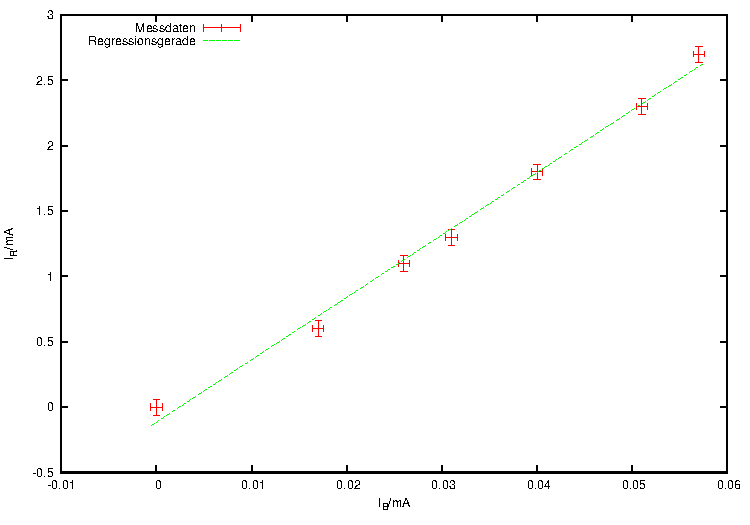
\includegraphics[scale = 0.7]{a_3_i.pdf}
  	\caption[Verhältnis zwischen Eingans- und Ausgangsstrom]{Verhältnis zwischen Eingans- und Ausgangsstrom}
  \label{fig:a_3_i}
\end{figure}


Bei dem Aufbau aus Abbildung \ref{fig:5} sollten auch wieder die Eigenschaften der Strom- und Spannungsverstärkung untersucht und mit den Ergebnissen zuvor verglichen werden. Die Differenz zwischen der Eingangs- und der Ausgangsspannung liegt bei den zwei Transistoren bei 1,25, dies ist etwa das Doppelte vom der zuvor bestimmten Wert.



\begin{figure}[H] 
  \centering
    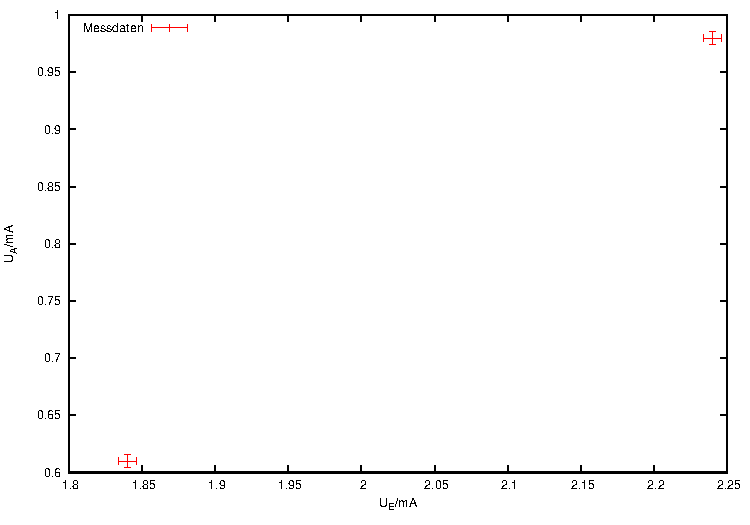
\includegraphics[scale = 0.7]{a_3b_u.pdf}
  	\caption[Verhältnis zwischen Eingans- und Ausgangsspannung]{Verhältnis zwischen Eingans- und Ausgangsspannung}
  \label{fig:a_3b_u}
\end{figure}

Die Stromverstärkung wurde wieder durch den Fit der Funktion f(x)=m$\cdot$x+b bestimmt. Dabei ergab sich f(x)=(0.0102$\pm$0.0005)$\cdot$x-(0.24$\pm$0.04). Also ergibt sich eine Verstärkung von 1,02$\cdot10^4$. Der Faktor $10^6$ kommt daher, dass im Plot mA gegen nA aufgetragen wurden. Die Stromverstärkung ist bei den zwei Transistoren also 200 mal größer.


\begin{figure}[H] 
  \centering
    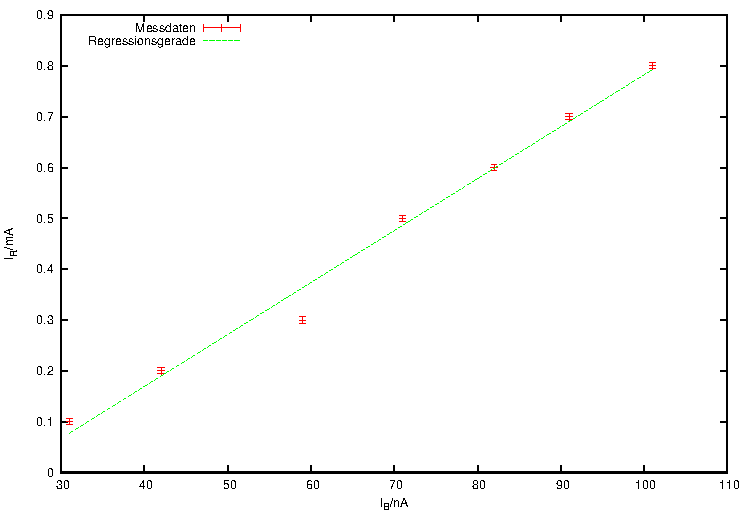
\includegraphics[scale = 0.7]{a_3b_i.pdf}
  	\caption[Verhältnis zwischen Eingans- und Ausgangsstrom]{Verhältnis zwischen Eingans- und Ausgangsstrom}
  \label{fig:a_3b_i}
\end{figure}

Im letztem Aufbau, siehe Abbildung \ref{fig:6} sollte noch einmal der Lautsprecher angeschlossen werden, auf dem Oszilloskop ergab sich dann der Verlauf in Abbildung \ref{fig:a_3c}. Zudem war deutlich ein Signal zu hören, dies liegt daran, dass viel höhere Ströme Fließen und die Leistung ausreichend groß ist.

\begin{figure}[H] 
  \centering
    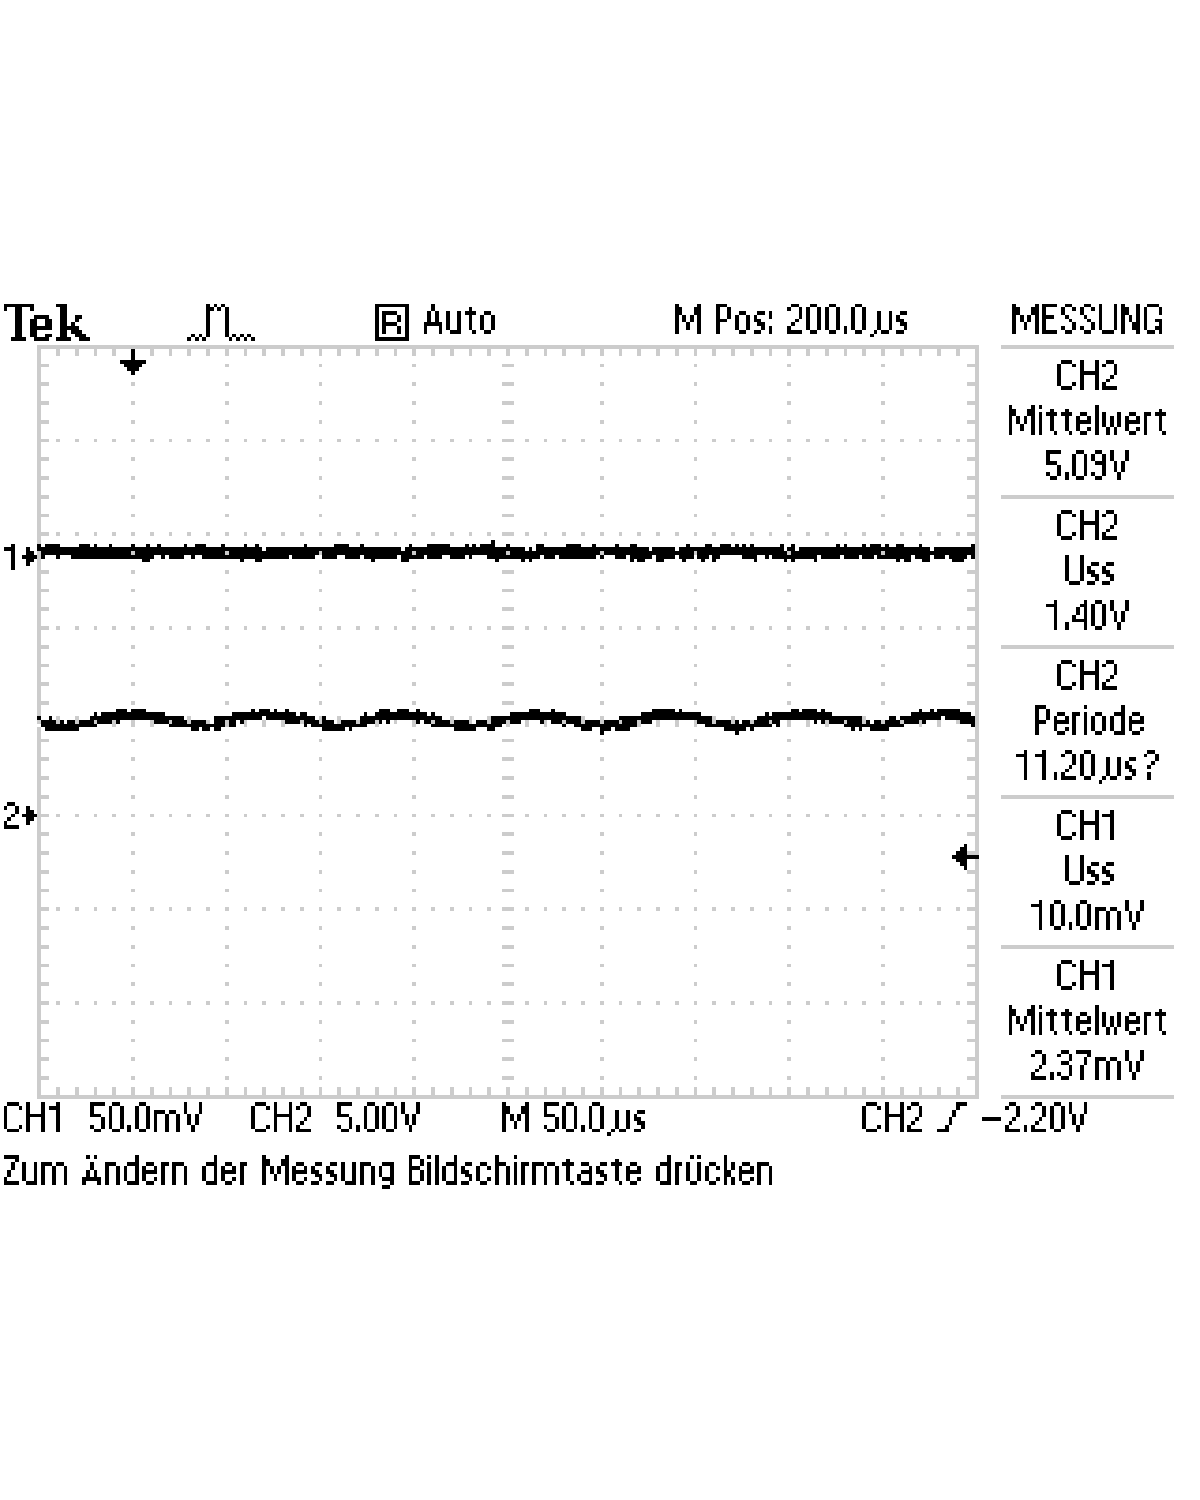
\includegraphics[scale = 0.7]{a_3c.pdf}
  	\caption[Verhältnis zwischen Eingans- und Ausgangsstrom]{Verhältnis zwischen Eingans- und Ausgangsstrom}
  \label{fig:a_3c}
\end{figure}

\subsection{Diskussion}
%(immer) die gemessenen werte und die bestimmten werte über die messfehler mit literaturwerten oder untereinander vergleichen
%in welchem fehlerintervall des messwertes liegt der literaturwert oder der vergleichswert?
%wie ist der relative anteil des fehlers am messwert und damit die qualität unserer messung?
%in einem satz erklären, wie gut unser fehler und damit unsere messung ist
%kurz erläutern, wie systematische fehler unsere messung beeinflusst haben könnten
%(wichtig) zum schluss ansprechen, in wie weit die ergebnisse mit der theoretischen vorhersage übereinstimmen
%--------------------------------------------------------------------------------------------
%falls tabellen mit den messwerten zu lang werden, kann die section mit den messwerten auch hinter der diskussion angefügt bzw. eine section mit dem anhang eingefügt werden.
%1-----------------------------------------------1
Im ersten Teil wurde ein Stromverstärkungsfaktor von $\beta$ 48 gemessen. Der Name der Schaltung Emitterfolger kommt daher, dass die Ausgangsspannung bzw. Emitterspannung der Eingangsspannung um 0.6 bis 0.7 Volt folgt. Diesen Effekt kann man an Abb. \ref{fig:a_3_u} gut beobachten. Entsprechend wurde bei der Darlingtonstufe der doppelte Effekt gemessen (Abb. \ref{fig:a_3b_u}). Da in diesem Aufbau Strom und Spannungsverstärkung zusammen geschaltet wurden konnte so eine ausreichend große Leistung erzeugt werden, sodass die Frequenzen deutlich über den Lautsprecher zu hören waren.


\section{Feldeffekttransistoren (FET)}
%kurz das ziel dieses versuchsteiles ansprechen, damit keine zwei überschriften direkt übereinander stehen!
%bei schwierigeren versuchen kann auch der theoretische hintergrund erläutert werden. (mit formeln, herleitungen und erklärungen)
Mit dem Feldeffekttransistor können Ströme und Spannungen fast leistungslos gesteuert werden. (Der Basisstrom beträgt nur wenige Nanoampere)
\subsection{Verwendete Geräte}
%(immer) eine skizze oder ein foto einfügen, die geräte/materialien !nummerieren! und z.b. eine legende dazu schreiben, besser wäre es das ganze in einem Fließtext gut zu beschreiben.
%falls am anfang des versuches nicht klar ist, was alles verwendet wird, wenn möglich erst am ende ein großes foto von den verwendeten materialien machen!\\

Für den Versuch wird ein Funktionsgenerator als Spannungsquelle, DMMs zur Messung, ein JFED Transistor und verschiedene Widerstände verwendet.

\subsection{Versuchsaufbau}
%skizze zum versuchsaufbau (oder foto) einfügen,   es muss erklärt werden wie das ganze funktioniert und welche speziellen einstellungen verwendet wurden (z.b. welche knöpfe an den geräten für die messung verdreht wurden)

\begin{itemize}
\item	J-FET BF224

\item	R1 10k$\Omega$

\item	R2 1k$\Omega$

\item	U1 10V
\end{itemize}

\begin{figure}[H] 
  \centering
    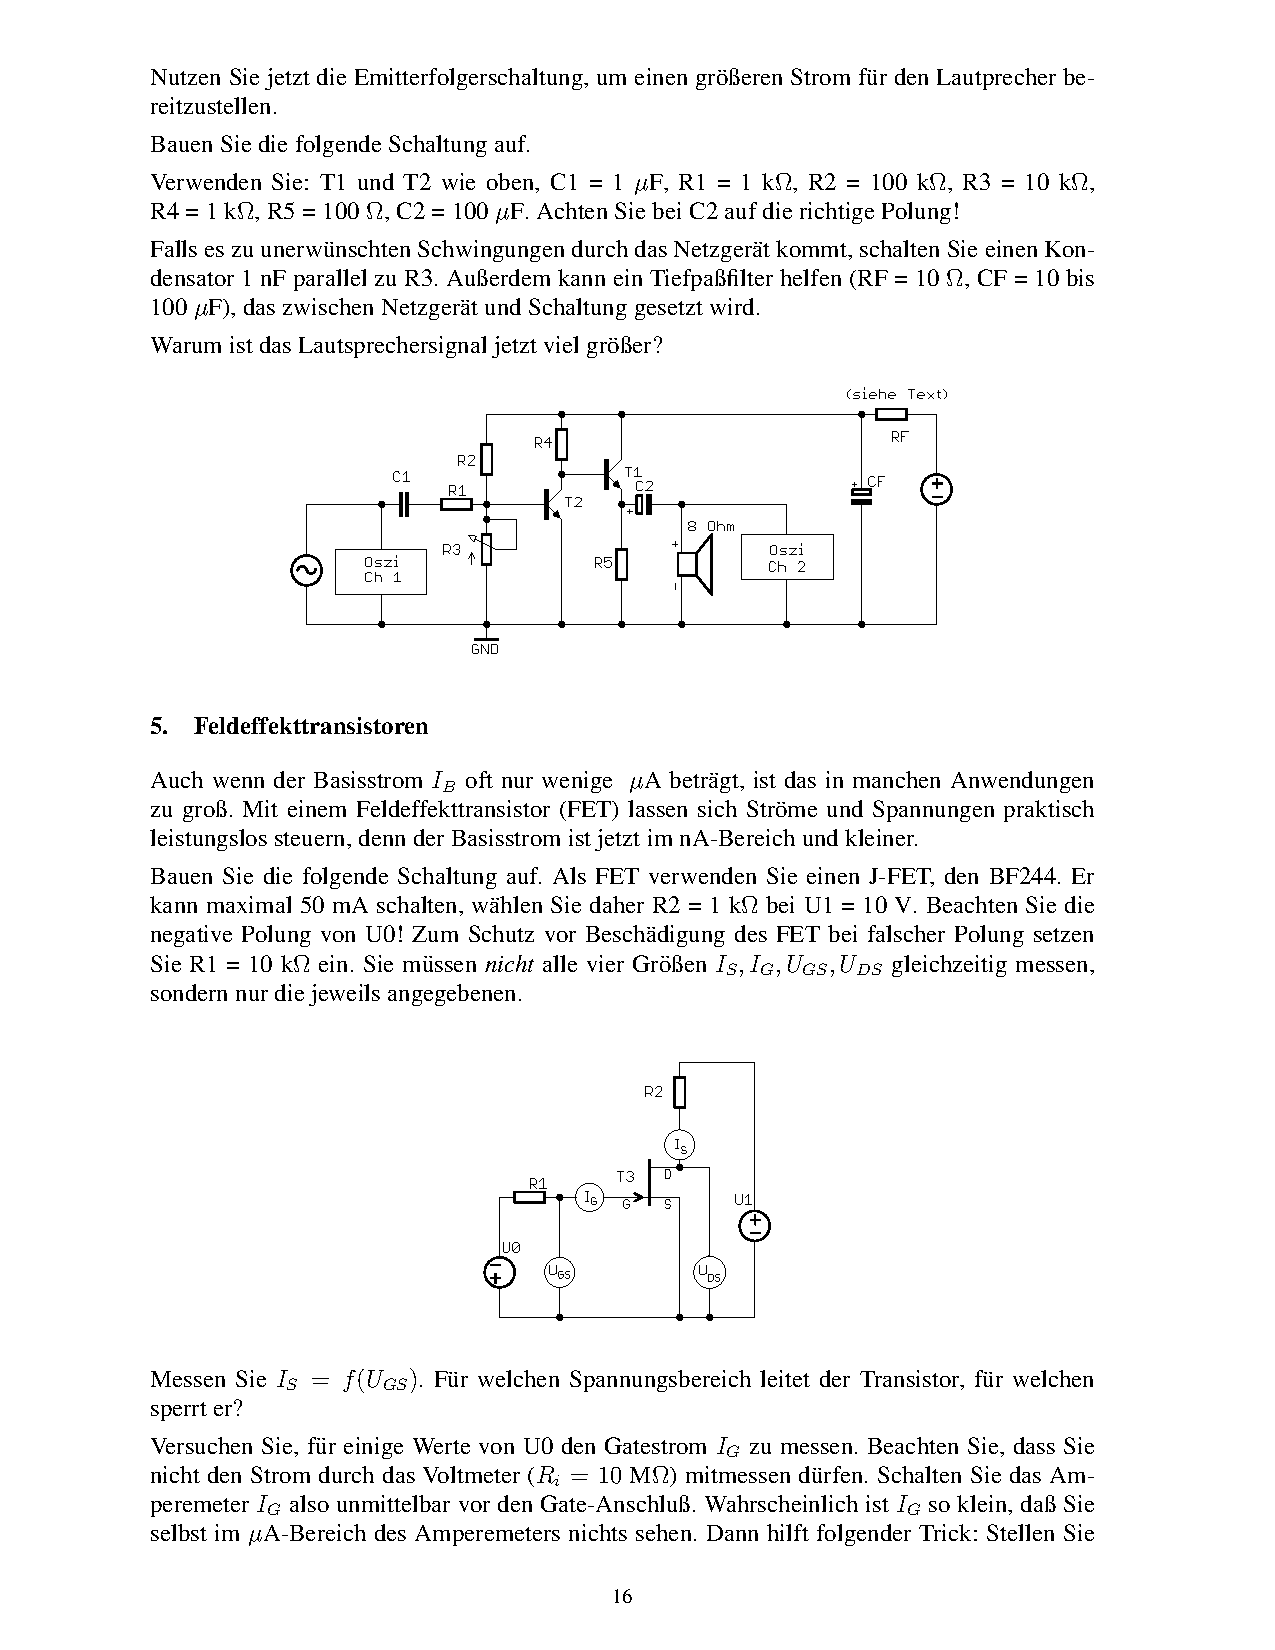
\includegraphics[trim = 10mm 50mm 10mm 174mm, clip, scale = 1]{ep3_14[Page16].pdf}
  	\caption[Schaltskizze für die Messung des Spannungsbereichs, in dem ein Feldaffekttransistor Leitet bzw. nicht]{Schaltskizze für die Messung des Spannungsbereichs, in dem ein Feldaffekttransistor Leitet bzw. nicht\footnotemark}
  \label{fig:7}
\end{figure}
\footnotetext{Abbildung entnommen von http://www.atlas.uni-wuppertal.de/$\sim$kind/ep3\_14.pdf Seite 16 am 10.11.2014}

\subsection{Versuchsdurchführung}
%erklären, !was! wir machen, !warum! wir das machen und mit welchem ziel
%(wichtig) präzize erklären, wie bei dem versuch vorgegangen und was gemacht wurde
Der Feldeffekttransistor kann über die Gatespannung $U_{GS}$ mit nur wenigen \unit{nA} angesteuert werden, sodass ein Feld entsteht, welches den Stromfluss $I_S$ reguliert. Dafür wird $I_S = f(U_{GS})$ ermittelt.
\subsection{Messergebnisse}
%die messwerte in !übersichtlichen! tabellen angegeben
%zu viele kleine tabellen in große tabellen überführen!
%zu große tabellen mit dem [scale]-befehl scalieren oder (falls zu lang) in zwei kleinere tabellen aufteilen
%(wichtig) vor !jeder! tabelle sagen, was gemessen wurde und wie die fehler gewählt wurden und ausreichend !erklären!, !warum! wir unsere fehler grade so gewählt haben

Der Fehler für den Strom und die Spannung wurde jeweils mit dem angegebenem Fehler und der Ableseungenauigkeit bestimmt, der Fehler der Spannung beträgt 0,006V und der Fehler des Stroms beträgt 0,06mA.

\begin{table}[htbp]
\caption{Messung von I$_\text{S}$ in Abhängigkeit von U$_\text{GS}$}
\begin{center}
\begin{tabular}{|r|r|}
\hline
U$_\text{GS}$/V & I$_\text{S}$/mA \\ \hline
0 & 7,8 \\ \hline
0,49 & 6,3 \\ \hline
1,06 & 4,2 \\ \hline
1,49 & 2,8 \\ \hline
2,03 & 1,2 \\ \hline
2,59 & 0,1 \\ \hline
3,03 & 0 \\ \hline
\end{tabular}
\end{center}
\label{tab:a_4}
\end{table}


\subsection{Auswertung}
%zuerst !alle! errechneten werte entweder in ganzen sätzen aufzählen, oder in tabellen (übersichtlicher) dargestellen, sowie auf die verwendeten formeln verweisen (die referenzierung der formel kann in der überschrift stehen)
%kurz erwähnen (vor der tabelle), warum wir das ganze ausrechnen bzw. was wir dort ausrechnen
%danach histogramme und plots erstellen, wobei wenn möglich funktionen durch die plots gelegt werden (zur not können auch splines benutzt werden, was aber angegeben werden muss)
%bei fits immer die funktion und das reduzierte chiquadrat mit angegeben, wobei auf verständlichkeit beim entziffern der zehnerpotenzen geachtet werden muss z.b. f(x)=(wert+-fehler)\cdot10^{irgendeine zahl}\cdot x + (wert+-fehler)\cdot10^{irgendeine zahl}
%bei jedem fit erklären, nach welchem zusammenhang gefittet wurde und warum!
%bei plots darauf achten, dass die achsenbeschriftung (auch die tics) die richtige größe haben und die legende im plot nicht die messwerte verdeckt
%kurz die aufgabenstellung abgehandeln
%2-----------------------------------------------2

Es sollte der Strom I$_\text{S}$ in Abhängigkeit von U$_\text{GS}$ gemessen werden und untersucht werden, ab welchem Spannungsbereich der Transistor anfängt zu sperren. Der Bereich liegt bei etwa 2,7V. 

\begin{figure}[H] 
  \centering
    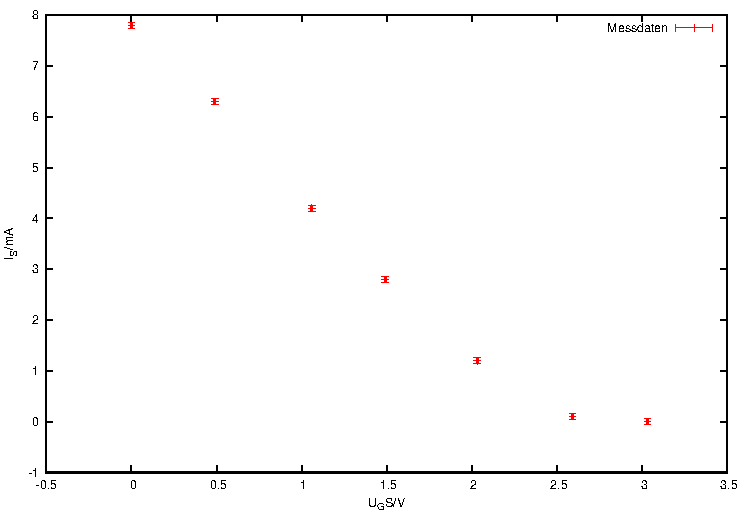
\includegraphics[scale = 0.7]{a_4.pdf}
  	\caption[Plot von I$_\text{S}$ in Abhängigkeit von U$_\text{GS}$]{Plot von I$_\text{S}$ in Abhängigkeit von U$_\text{GS}$}
  \label{fig:a_4}
\end{figure}

Beim Messen des Gatestrom konnten keine Werte aufgenommen werden, da die Ströme geringer als das Auflösungsvermögen des DMMs waren, obwohl der Trick aus der Praktikumsanleitung verwendet wurde.

\subsection{Diskussion}
%(immer) die gemessenen werte und die bestimmten werte über die messfehler mit literaturwerten oder untereinander vergleichen
%in welchem fehlerintervall des messwertes liegt der literaturwert oder der vergleichswert?
%wie ist der relative anteil des fehlers am messwert und damit die qualität unserer messung?
%in einem satz erklären, wie gut unser fehler und damit unsere messung ist
%kurz erläutern, wie systematische fehler unsere messung beeinflusst haben könnten
%(wichtig) zum schluss ansprechen, in wie weit die ergebnisse mit der theoretischen vorhersage übereinstimmen
%--------------------------------------------------------------------------------------------
%falls tabellen mit den messwerten zu lang werden, kann die section mit den messwerten auch hinter der diskussion angefügt bzw. eine section mit dem anhang eingefügt werden.
%1-----------------------------------------------1

Im ersten Teil sollte überprüft werden ab welcher Spannung U$_\text{GS}$ der Strom I$_\text{S}$ gesperrt wird, dabei ergab sich ein Spannung von 2,7V.Zudem sollte noch der Gatestrom gemessen werden, wobei sehr kleine Werte für den Gatestrom erwartet wurde. Der Gatestrom war so klein, dass er mit den Messapparaturen nicht zu messen war.

\section{Spannungsstabilisierung mit Transistoren}
%kurz das ziel dieses versuchsteiles ansprechen, damit keine zwei überschriften direkt übereinander stehen!
%bei schwierigeren versuchen kann auch der theoretische hintergrund erläutert werden. (mit formeln, herleitungen und erklärungen)
Analog zum letzten Versuch kann mit einer Zenerdiode eine konstante Gleichspannung erzeugt werden. Aufgrund des Vorwiderstandes war es aber nicht möglich hohe Ausgangsströme zu erreichen. Führt man die Zehnerspannung über einen Emittierfolger (Stromverstärker), so sind wesentlich höhere Ströme möglich.
\subsection{Verwendete Geräte}
%(immer) eine skizze oder ein foto einfügen, die geräte/materialien !nummerieren! und z.b. eine legende dazu schreiben, besser wäre es das ganze in einem Fließtext gut zu beschreiben.
%falls am anfang des versuches nicht klar ist, was alles verwendet wird, wenn möglich erst am ende ein großes foto von den verwendeten materialien machen!\\

Bei dem Versuch wurde ein Funktionsgenerator für die Spannungsversorgung, DMMs, eine Zenerdiode, eine Transistor, ein Widerstand, ein Kondensator und ein Potentiometer verwendet.

\subsection{Versuchsaufbau}
%skizze zum versuchsaufbau (oder foto) einfügen,   es muss erklärt werden wie das ganze funktioniert und welche speziellen einstellungen verwendet wurden (z.b. welche knöpfe an den geräten für die messung verdreht wurden)

\begin{itemize}
\item	D1 Zenerdiode

\item	T1 BD137

\item	R1 200$\Omega$

\item	R2 470$\Omega$ Potentiometer

\item	R3 = 20$\Omega$

\item	100nF
\end{itemize}

\begin{figure}[H] 
  \centering
    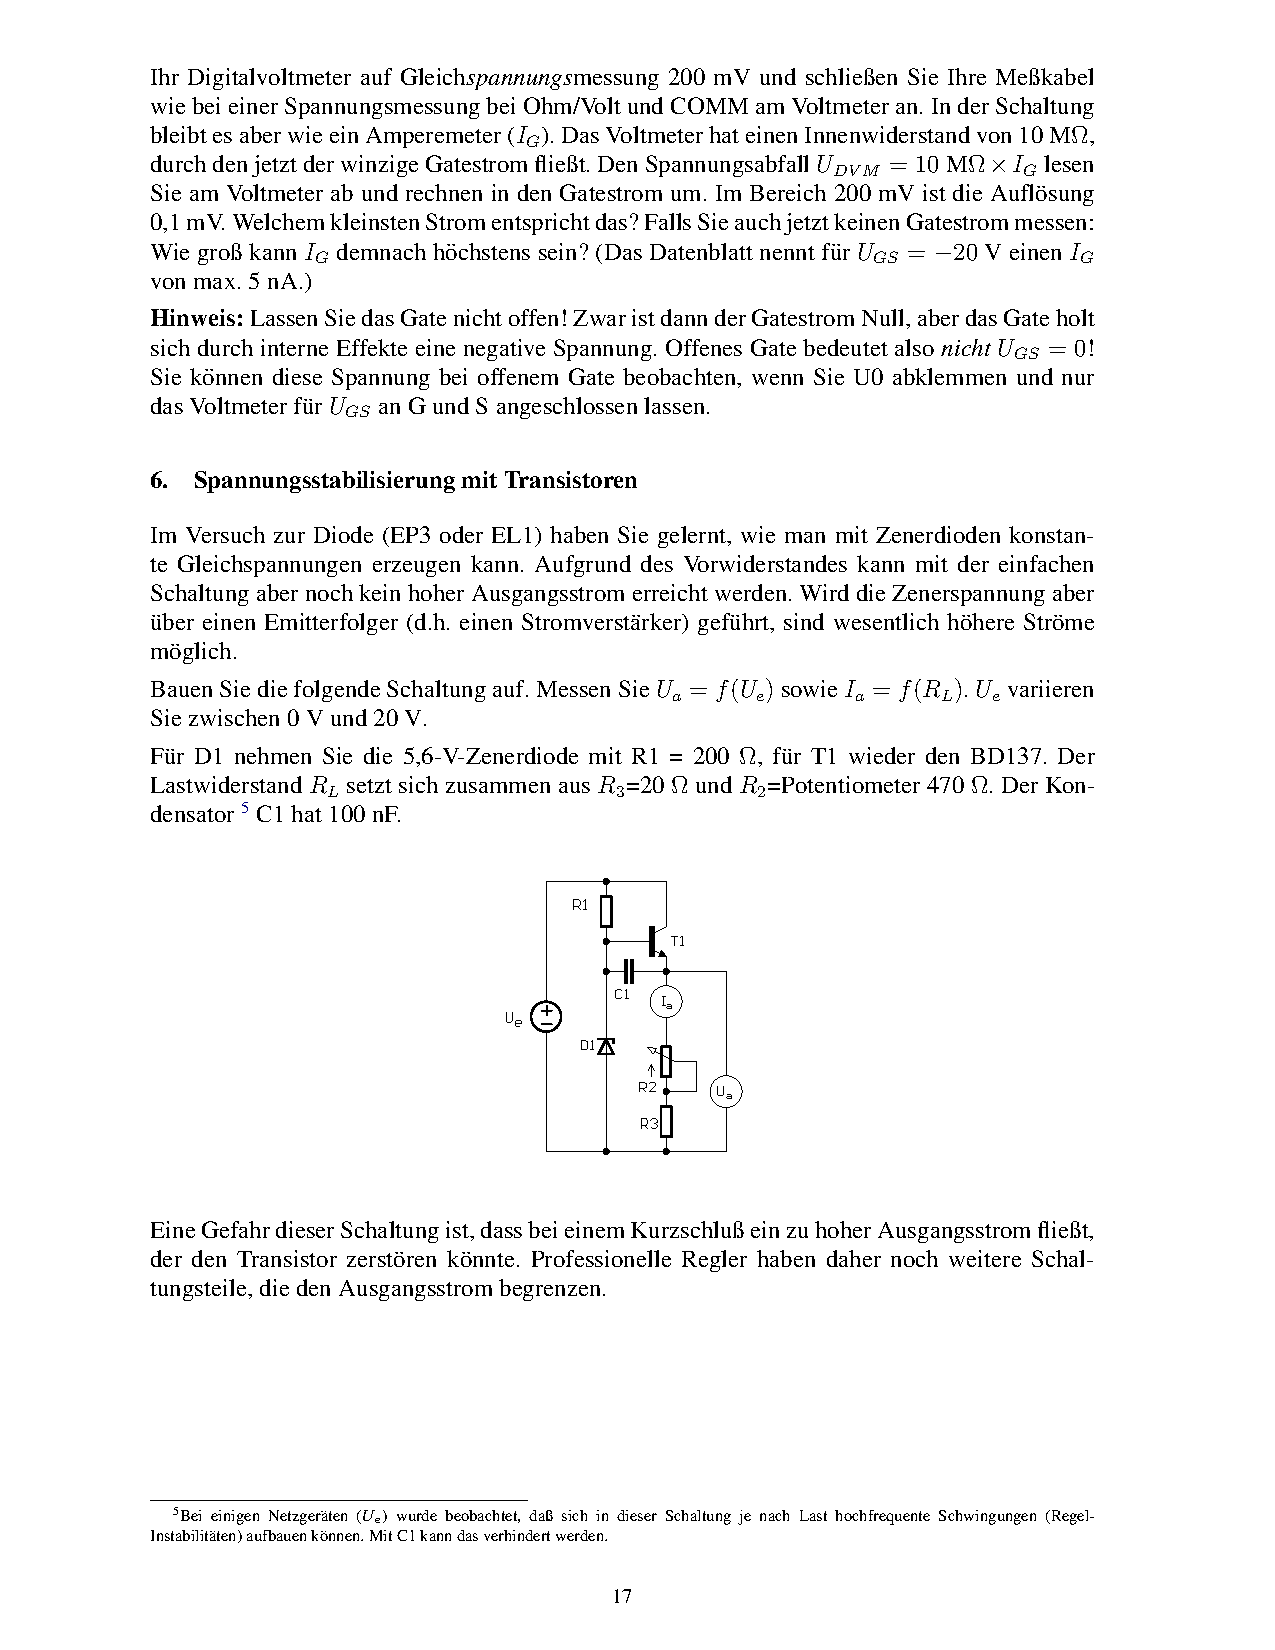
\includegraphics[trim = 10mm 80mm 10mm 140mm, clip, scale = 1]{ep3_14[Page17].pdf}
  	\caption[Schaltskizze für die Messung der Spannungsstabilisierung durch Transistoren]{Schaltskizze für die Messung der Spannungsstabilisierung durch Transistoren\footnotemark}
  \label{fig:8}
\end{figure}
\footnotetext{Abbildung entnommen von http://www.atlas.uni-wuppertal.de/$\sim$kind/ep3\_14.pdf Seite 16 am 10.11.2014}

\subsection{Versuchsdurchführung}
%erklären, !was! wir machen, !warum! wir das machen und mit welchem ziel
%(wichtig) präzize erklären, wie bei dem versuch vorgegangen und was gemacht wurde
Wie im letzten Praktikumsversuch zur Diode wird in diesem Versuchsteil auch eine Zenerdiode zur Spannungsstabilisierung verwendet. Der Unterschied in dieser Schaltung (Abb. \ref{fig:8}) ist die Verwendung eines Transistors zur Verstärkung des Stroms durch die Last um eine größere Leistung zu ermöglichen. Da am Transistor im Arbeitspunkt immer ca. 0.7 V abfallen, ist die Spannung, welche an der Last abfällt auf \unit[5]{V} begrenzt.
\subsection{Messergebnisse}
%die messwerte in !übersichtlichen! tabellen angegeben
%zu viele kleine tabellen in große tabellen überführen!
%zu große tabellen mit dem [scale]-befehl scalieren oder (falls zu lang) in zwei kleinere tabellen aufteilen
%(wichtig) vor !jeder! tabelle sagen, was gemessen wurde und wie die fehler gewählt wurden und ausreichend !erklären!, !warum! wir unsere fehler grade so gewählt haben

Der Fehler für die Eingangsspannung wurde mit dem Ablesefehler angenommen und beträgt 0,1V, der Fehler der Ausgangsspannung wurde aus dem angegebenen Fehler und der Ableseungenauigkeit bestimmt und beträgt 0,06V.

\begin{table}[H]
\caption{Messung von U$_\text{A}$ in Abhängigkeit von U$_\text{E}$}
\begin{center}
\begin{tabular}{|r|r|}
\hline
U$_\text{E}$/V & U$_\text{A}$/V \\ \hline
0 & 0 \\ \hline
2 & 1,33 \\ \hline
4 & 3,22 \\ \hline
6 & 4,22 \\ \hline
8 & 4,36 \\ \hline
10 & 4,41 \\ \hline
12 & 4,44 \\ \hline
14 & 4,48 \\ \hline
16 & 4,5 \\ \hline
18 & 4,55 \\ \hline
20 & 4,58 \\ \hline
\end{tabular}
\end{center}
\label{tab:a_5_u}
\end{table}

Die Fehler wurden jeweils mit dem angegebenem Fehler und der Ableseungenauigkeit bestimmt, dabei ergab sich ein Fehler von 6$\Omega$ für R$_\text{L}$ und ein Fehler von 0,6mA für den Strom.

\begin{table}[H]
\caption{Messung von I$_\text{A}$ in Abhängigkeit von R$_\text{L}$}
\begin{center}
\begin{tabular}{|r|r|}
\hline
R$_\text{L}$/$\Omega$ & I$_\text{G}$/mA \\ \hline
567 & 7 \\ \hline
503 & 7,8 \\ \hline
433 & 9 \\ \hline
370 & 10,6 \\ \hline
322 & 12 \\ \hline
280 & 13,8 \\ \hline
240 & 16 \\ \hline
200 & 19 \\ \hline
170 & 22,1 \\ \hline
140 & 26,4 \\ \hline
100 & 35,7 \\ \hline
70 & 49,5 \\ \hline
\end{tabular}
\end{center}
\label{tab:a_5_i}
\end{table}



\subsection{Auswertung}
%zuerst !alle! errechneten werte entweder in ganzen sätzen aufzählen, oder in tabellen (übersichtlicher) dargestellen, sowie auf die verwendeten formeln verweisen (die referenzierung der formel kann in der überschrift stehen)
%kurz erwähnen (vor der tabelle), warum wir das ganze ausrechnen bzw. was wir dort ausrechnen
%danach histogramme und plots erstellen, wobei wenn möglich funktionen durch die plots gelegt werden (zur not können auch splines benutzt werden, was aber angegeben werden muss)
%bei fits immer die funktion und das reduzierte chiquadrat mit angegeben, wobei auf verständlichkeit beim entziffern der zehnerpotenzen geachtet werden muss z.b. f(x)=(wert+-fehler)\cdot10^{irgendeine zahl}\cdot x + (wert+-fehler)\cdot10^{irgendeine zahl}
%bei jedem fit erklären, nach welchem zusammenhang gefittet wurde und warum!
%bei plots darauf achten, dass die achsenbeschriftung (auch die tics) die richtige größe haben und die legende im plot nicht die messwerte verdeckt
%kurz die aufgabenstellung abhandeln
%2-----------------------------------------------2

In Abbildung \ref{fig:a_5_u} ist zu erkennen wie die Ausgangsspannung ab einer Eingangspannung von 5V stabilisiert wird. In Abbildung \ref{fig:a_5_i} kann man sehen, dass der Strom vom Lastwiderstand und von der Kennlinie des Emitters abhängt.
\begin{figure}[H]
\begin{subfigure}{0.49\textwidth}
  \centering
    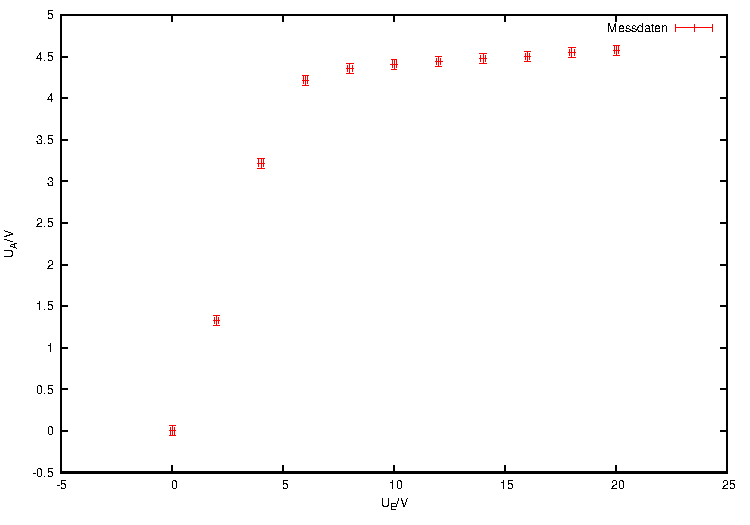
\includegraphics[scale = 0.7]{a_5_u.pdf}
  	\caption[Plot von U$_\text{A}$ in Abhängigkeit von U$_\text{E}$]{Plot von U$_\text{A}$ in Abhängigkeit von U$_\text{E}$}
  \label{fig:a_5_u}
\end{subfigure}
\hfill
\begin{subfigure}{0.49\textwidth}
  \centering
    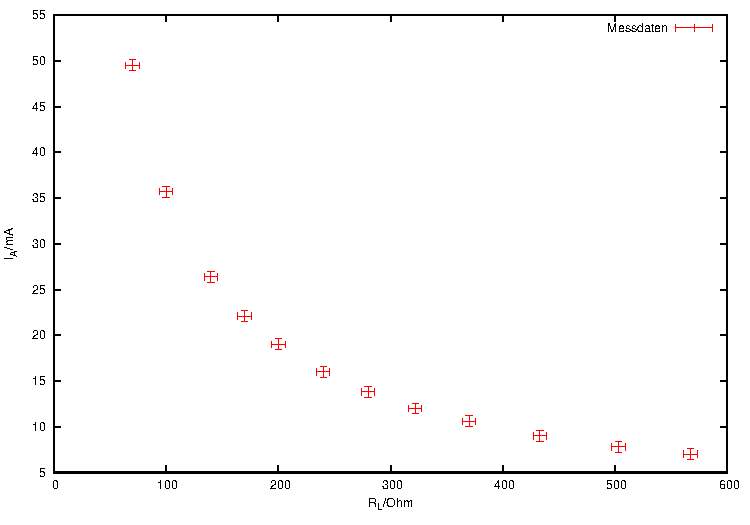
\includegraphics[scale = 0.7]{a_5_i.pdf}
  	\caption[Plot von I$_\text{S}$ in Abhängigkeit von R$_\text{L}$]{Plot von I$_\text{A}$ in Abhängigkeit von R$_\text{L}$}
  \label{fig:a_5_i}
\end{subfigure}
\caption{Plot der Ausgangsspannung gegen die Eingangsspannung und des Stromes gegen den Lastwiderstand}
\end{figure}


\subsection{Diskussion}
%(immer) die gemessenen werte und die bestimmten werte über die messfehler mit literaturwerten oder untereinander vergleichen
%in welchem fehlerintervall des messwertes liegt der literaturwert oder der vergleichswert?
%wie ist der relative anteil des fehlers am messwert und damit die qualität unserer messung?
%in einem satz erklären, wie gut unser fehler und damit unsere messung ist
%kurz erläutern, wie systematische fehler unsere messung beeinflusst haben könnten
%(wichtig) zum schluss ansprechen, in wie weit die ergebnisse mit der theoretischen vorhersage übereinstimmen
%--------------------------------------------------------------------------------------------
%falls tabellen mit den messwerten zu lang werden, kann die section mit den messwerten auch hinter der diskussion angefügt bzw. eine section mit dem anhang eingefügt werden.
%1-----------------------------------------------1
Indem ein Transistor in die Schaltung zur Spannungsstabilisierung eingebaut wurde, konnte an der Last eine größere Leistung abgenommen werden. Man sieht an Abb. \ref{tab:a_5_u} das die Spannung an der Last durch die Zenerdiode auf \unit[5]{V} beschränkt ist. Da in dieser Schaltung der Vorwiderstand parallel zum Transistor geschaltet werden kann, und nur ein geringer Strom durch diesen fließen muss, um den Arbeitspunkt des Transistors einzustellen, fällt fast keine Leistung am Vorwiderstand ab. Der Basisstrom wird sogar um den Faktor $\beta$ verstärkt, sodass am Lastwiderstand eine höhere Leistung erzielt werden kann. 
\section{Fazit}
%im fazit nochmal alles zusammenfassen und den verlauf der messung abschätzen
%gravierende sytematische probleme bei den messungen nochmal betonen und die wertigkeit unserer ergebnisse einordnen

Der erste Versuchsteil verlief gut und die aufgenommenen Kurven entsprachen alle den Erwartungen. Im zweitem Versuchsteil wurde mit einem Transistor eine Spannungsverstärkung durchgeführt und ein Verstärkung von 100 erreicht, jedoch konnte durch den Spannungsteiler nicht genug Leistung abgegriffen werden, um einen Lautsprecher zu betreiben. Aus diesem Grund wurde im dritten Versuchsteil eine 	Darlingtonstufe verwendet. Dadurch fand eine Strom- und Spannungsverstärkung statt und es wurde genügend Leistung geliefert, um den Lautsprecher zu betreiben. Im viertem Versuchsteil wurde die Eigenschaft eines JFEDs untersucht, den Strom zu sperren. Es wurde eine Spannung von 2,7V gemessen, ab der der Strom gesperrt wurde. Im letztem Versuchsteil wurde ein Transistor zur Spannungsstabilisierung verwendet wo deutlich eine Stabilisierung zu erkennen war.
Durch die Versuche lies sich der Nutzen von Transistoren zur Spannung- und Stromverstärkung und Stabilisierung in Schaltnetzwerken zeigen.

\end{document}

